\documentclass{classeENS}
\usepackage{lipsum}
\usepackage[backend=bibtex,style=alphabetic,natbib=true]{biblatex} % Use the bibtex backend with the authoryear citation style (which resembles APA)
\addbibresource{biblio.bib} % The filename of the bibliography
\usepackage[autostyle=true]{csquotes} % Required to generate language-dependent quotes in the bibliography

\usepackage{algorithm}
\usepackage{algorithmicx}
\usepackage{algpseudocode}
\usepackage{amsmath}
\usepackage{amssymb}
\usepackage{comment}
\usepackage{mathtools, stmaryrd}
\usepackage{parskip}
\usepackage{titlesec}
\usepackage{tikz}
\usepackage{listings}
\usepackage{xcolor}

\definecolor{codegreen}{rgb}{0,0.6,0}
\definecolor{codegray}{rgb}{0.5,0.5,0.5}
\definecolor{codepurple}{rgb}{0.58,0,0.82}
\definecolor{backcolour}{rgb}{0.95,0.95,0.92}

\lstdefinestyle{mystyle}{
    backgroundcolor=\color{backcolour},   
    commentstyle=\color{codegreen},
    keywordstyle=\color{magenta},
    numberstyle=\tiny\color{codegray},
    stringstyle=\color{codepurple},
    basicstyle=\ttfamily\footnotesize,
    breakatwhitespace=false,         
    breaklines=true,                 
    captionpos=b,                    
    keepspaces=true,                 
    numbers=left,                    
    numbersep=5pt,                  
    showspaces=false,                
    showstringspaces=false,
    showtabs=false,                  
    tabsize=2
}

\lstset{style=mystyle}

\setcounter{secnumdepth}{4}
\setcounter{tocdepth}{3}
\makeatletter
\newcounter{subsubsubsection}[subsubsection]
\renewcommand\thesubsubsubsection{\thesubsubsection .\@alph\c@subsubsubsection}
\newcommand\subsubsubsection{\@startsection{subsubsubsection}{4}{\z@}%
                                     {-3.25ex\@plus -1ex \@minus -.2ex}%
                                     {1.5ex \@plus .2ex}%
                                     {\normalfont\normalsize\bfseries}}
\newcommand*\l@subsubsubsection{\@dottedtocline{3}{10.0em}{4.1em}}
\newcommand*{\subsubsubsectionmark}[1]{}
\makeatother

\usepackage{array,multirow,makecell}
\setcellgapes{1pt}
\makegapedcells
\newcolumntype{R}[1]{>{\raggedleft\arraybackslash }b{#1}}
\newcolumntype{L}[1]{>{\raggedright\arraybackslash }b{#1}}
\newcolumntype{C}[1]{>{\centering\arraybackslash }b{#1}}
\newcolumntype{M}[1]{>{\centering}m{#1}}

\setlist[itemize]{label=\textbullet}

\title{Template rapport ENS} %Titre du fichier

\begin{document}

%----------- Informations du rapport ---------

\titre{Internship report} %Titre du fichier .pdf
\departement{Computer Graphics} 
\matiere{} 
\motif{}

\enseignant{Nicolas \textsc{Bonneel}\\
            Jean-Claude \textsc{Ielh}} %Nom de l'enseignant
\tuteurpcp{}
\eleves{Pacôme \textsc{Luton}} %Nom des élèves

%----------- Initialisation -------------------
        
\fairemarges %Afficher les marges

%\fairepagedegarde

\tabledematieres %Créer la table de matières
%\tabledefigure

%------------ Corps du rapport ----------------
\section{Introduction}

This work is an invitation to the journey I followed during my internship. 

\par In 3D rendering, we want to render images. To so, for each pixel 
we simulate photon paths that goes from a light, bounce on object and finally 
arrive in the sensor of the camera.

{\color{red} TODO : Add a schema of photon path}

\par This is equivalent to computing a multidimensional integral numerically. 
In the general case this is a difficult problem. Often the best we can do is 
to compute an approximation of the integral. This is done by Monte Carlo 
integration. I will describe this method in the preliminaries \ref{montecarlo}, 
but intuitively this method corresponds to simulating a certain 
number of photon paths. And the more photons simulated, the better 
the approximation to the true integral.

\par Simply put, we have to do a Monte Carlo numerical integration for each pixel 
of the image. And each numerical integration converges more or less quickly. 
For example, if a pixel corresponds to a light, we have a good approximation 
of the integral directly with a single photon path. But for a pixel that represents a dark 
region under a table, we have to simulate several photon paths to take into account
all the global illumination and have a good approximation of the true integral.

\par In practice, each photon path costs a certain amount of computing power. 
And we want to render the image (find a good approximation of the integral 
for each pixel) with the minimum number of computations. So a simple idea 
to reduce the number of computations is to allocate a different number 
of computationnal power (number of photon paths) to each pixel. This is called 
adaptive sampling. This idea was introduced very early in the 
history of computer graphics \cite{10.1145/325165.325179}.

\par The goal of this internship was to explore new ways of doing adaptive 
sampling, with a small quantity of information.
%-------------------------------------------------------------------------
\section{Preliminaries}

\begin{figure}[H]
    \centering
    \begin{tabular}{C{2cm} L{10cm}}
    \hline  
        Symbol & Description
    \tabularnewline 
    \hline
        $X$ & scene
    \tabularnewline
        $X_n$ & render of a scene with $n$ spp
    \tabularnewline
        $\mathbb E(\cdot)$ & expectation
    \tabularnewline
        $\mathbb V(\cdot)$ & variance
    \tabularnewline
        $\R$ & renderer function
    \tabularnewline
        $\Sm$ & sampling map function
    \tabularnewline
        $\D$ & denoiser function
    \tabularnewline
        $\Los$ & loss function
    \tabularnewline
        $(a,b)$ & convergence rate of the error $e = b/n^a$
    \tabularnewline
    \hline 
    \end{tabular}
\end{figure}

\subsection{Monte Carlo Integration}

\subsubsection{Definition}\label{montecarlo}

Monte Carlo integration is an approximation $I_N$ of the integral 
$I$ of $f$ on the domain $\mathbb A$ by evaluating $f$ in $N$ \textbf{independant} 
random points $\{x_j\}_{j=1}^N$ uniformly distributed over the 
space $\mathbb A$. Formally:
\begin{equation}
    \label{eq:montecarlo}
    I_N = \int_{\mathbb A} S(x)f(x)dx, 
        \: \text{ with } \:
    S(x) = \frac{1}{N} \sum_{j=1}^N \delta(\lVert x-x_j \rVert)
\end{equation}
We know that the mean and the variance of our estimation are:
\begin{equation}
    \E(I_n) = I(f) \quad \text{and} \quad \V(I_N) = \frac{Var(f)}{N}
\end{equation}
where $I(f)$ is the true integral of $f$, and $Var(f)$ is the variation of $f$. 
The variance is really important as the error in the integration is directly 
linked to the variance as
\begin{align*}   \label{eq:variance}
    \E((I(f) - I_N)^2) = \E((E(I_N) - I_N)^2) = \V(I_N)
\end{align*}

\subsubsection{Stratified sampling}

A technique to reduce the error, is to do a variante of Monte Carlo Integration, 
called Quasi-Monte Carlo. Instead of taking $N$ \textbf{independant} random points $\{x_j\}_{j=1}^N$ 
uniformly distributed over the space $\mathbb A$, we take $N$ \textbf{correlated} random 
points $\{x_j\}_{j=1}^N$ uniformly distributed over the space $\mathbb A$. Formally, 
the variance of the estimator is now:
 
\[ \V(I_N) = \V\left [\frac{1}{N}\sum_{j=1}^N f(x_j) \right ] = \frac{Var(f)}{N} + \frac{2}{N}\sum_{i\neq j} CoVar(f(x_i),f(x_j)) \]

By a well chosen correlation, we hope that this will reduce the variance of our estimator and so the error
of our estimation. 

\par One of the known way of generate a good correlation, is to use stratified sample, like 
a Sobol sequence, Halton sequence or Hammersley Sequence. The idea
of stratified sampling is to distribute the sample all over the space.

For simple integrals, the stratified sampler gives provably lower error and 
faster asymptotic convergence \cite{10.1145/237170.237265}. And empirically,
stratified samplers also give better rate of convergence for complex integrals that
occur in rendering \cite{renderman}.

\paragraph*{Summary} What is important to remember to understand this work is that 
in order to reduce the error, most of the modern renderer use a stratified sequence like 
Sobol \cite{renderman} to produce random points. And those random points are correlated.

\subsection{Adaptative Sampling}

\par Let $P$ be the number of pixels in the image and, $I^{(p)}$ the integral of the pixel $p$. 
When producing an image, we have $P$ integral to compute, one for each pixel, and we have a
global budget $B$ that correspond the total number sample we will compute in the entire 
image. And as simulating a photon path (caracterized by the sample) take about the 
same time, it is equivalent to limit the time we have to render the image.

\par Usually, $B=n\times P$ and we use $n$ sample to approximate each integral $I^{(p)}$.
But as each numerical integration converge to a different rate, we may improve the global error
(the sum of the error of each pixel) by using a different number of sample in for each pixel,
but with still the same global budget $B$.
\par Formally, for a budget $B$, we called a sampling map the gray scale image $n$, 
where $n_p$ is the number of sample used to approximate $I^{(p)}$. The sampling 
satisfy $\sum_{p} n_p = B$. Here is what a typical sampling map looks like:

\begin{figure}[H]
    \centering
    \caption{Example of a sampling map}
    \begin{tabular}{cc}
    \includegraphics[width=45mm]{image/without/gt.png}
    & 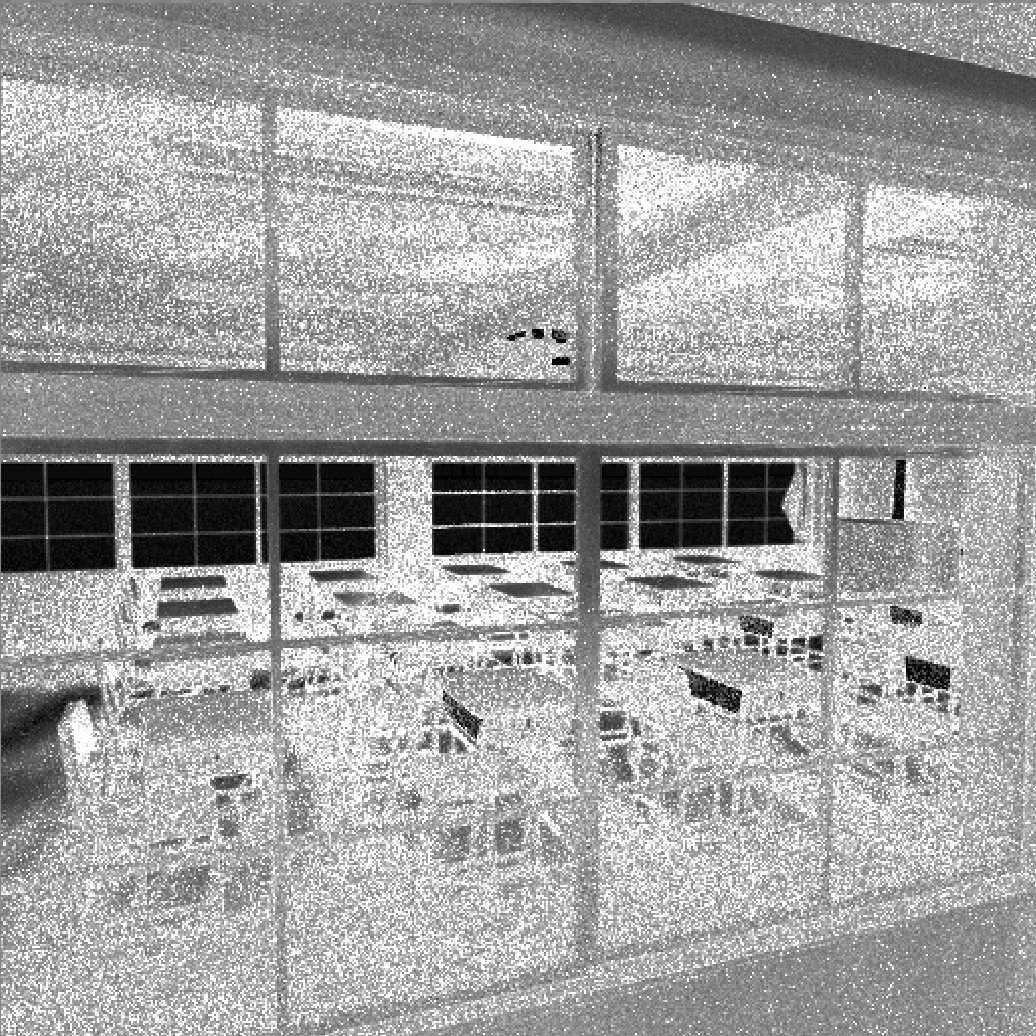
\includegraphics[width=45mm]{image/without/sm.png}\\
    the image & a sampling map
    \end{tabular}
\end{figure}


\par The one million dollar question is then, for a scene $X$, how to find the optimal
sampling map $n$. Before explaining what is an optimal sampling, let introduce our notation:
\begin{itemize}
    \item $B$ is the global budget, corresponding to the total number photon path simulated
    in order to render the image.
    \item $n$ is a sampling map. It's a gray scale image, where each pixel value $n_p$, is the
    number of sample that is used to numerically integrate the integrale $I^{(p)}$. In this paper,
    for $m$ integer, will note $\bar m$ the sampling map where $n_p = m$ for all $p$.
    \item $\R$ is the renderer. It take as input a scene $X$ and a sampling map $n$ and it produce
    a possible final image $X_n$. One thing that is important, is that the final image $X_n$ is a 
    stochastic process. In this paper, we really see $\R(X,n)$ 
    as a random variable parameterized by the scene $X$ and the sampling map $n$.
    \item $\Sm$ is the function we're intrested in. We will called it the sampling function. 
    It take as input a scene $X$, and a rendered image $X_{\bar m}$ with a small number 
    of sample ($m$ is relatively small compare to global budget $B$), and it produce a sampling map $n$.
    We will note $\Sm_{uni}$ the sampling function that always outputs $\bar m$.
    \item $\D$ is the denoiser function, that take as input a rendered image $X_n$ and try to
    denoise it in order to reduce the error.
    \item $\Los$ is the loss function, it take as input the rendered image $X_n$ and the groundtruth 
    image $X_\infty$ and outputs the error. In this paper it's the Relative Mean Square Error (RMSE).
\end{itemize}
With those notation, we can formalize what is an optimal sampling map, for a given scene, 
the optimal sampling $n_{opt}$ is:
\begin{equation}
    \label{eq:0}
    n_{opt} = \argmin_{n_{opt}} \E \left [ \Los (\D (\R(X, n)), I_\infty) \right ]
\end{equation}
Note that is an expectation as the renderer is a random variable. We want to minimise the 
expectation of the error.

\par And we can also try to formalize what is an optimal sampling function $\Sm_{opt}$.
Given an arbritrary set of scenes $\Omega$, possibly infinite, $\Sm_{opt}$ on this set of 
scenes is:
\begin{equation}
    \label{eq:1}
    \Sm_{opt} = \argmin_{\Sm} \int_{I\in\Omega} \E \left [ \Los (\D (\R(X, \Sm(X_n, B))), I_\infty) \right ]
\end{equation}

The goal of this intership was notably to find good sampling function, as close as 
possible as the optimal sampling function. But before, let's looks at the state of the art.

\subsection{State of the art}

In the state of the art, I see two main categorie of way of finding good sampling function:
\begin{itemize}
    \item Techniques that use a prior knowledge on what should look like a good sampling map, 
    and use it to build a good sampling function.
    \item Techniques that optimise simply the equation \ref{eq:1} by gradient descent.
\end{itemize}
I will describe shortly how some of those method work, and their weakness.

\subsubsection{Using prior knowledge}

\par The idea is that we have a prior knowledge on what should look like a good 
sampling map. For example, as we know that the error in Monte Carlo 
is directly proportionnal to the variance of the function \label{eq:variance},
we can used this fact to try to have a good sampling map \cite{10.1145/325165.325179}.

\par But this method, that work in Monte Carlo integration, is not designed for
Quasi-Monte Carlo integration that use stratified sample. It doesn't take the 
covariance term into account. 
And as we have seen previously, most of the modern renderer use stratified sample. 

\paragraph*{Perspective} Thus it will be great if we had a method close to this one that take into account
the fact that we use stratified sample. This is the problem on which I work on during the first
part of my intership.

\subsubsection{With optimisation}

In 2018, \cite{kuznetsov2018deep} propose to approximate $S_{opt}$ by doing a stochastic
gradient descent on the space of convolutional neural networks. In the same time they also 
optimise the denoiser to work well with the sampler, but it's not what is really important. 
Formmaly, they are optimising an equation that is slightly different from \ref{eq:1}:
\begin{equation}
    \label{eq:2}
    \D_{opt}, \Sm_{opt} = \argmin_{D, \Sm} \int_{X\in\Omega} \E_r \left [ \Los (\D (\R(X, \Sm(X_n, B), r)), X_\infty) \right ]
\end{equation}

\paragraph*{Problem} In order to optimise the equation \ref{eq:2} by gradient descent,
we need to be able to evaluate $\R(X,s)$ quickly, which is impossible for most scenes.
And we also need to be able to compute $\frac{\partial \R}{\partial s}$, where $s$ is a 
sampling map.


\par To solve this problem, \cite{kuznetsov2018deep} introduced a pipeline to still optimise
the equation. The idea is to train on a slightly different from equation \ref{eq:2} and hope 
that the solution found will also work on the equation \ref{eq:1}.
\begin{equation}
    \label{eq:3}
    \D_{opt}, \Sm_{opt} = \argmin_{D, \Sm} \int_{X\in\Omega} \E_r \left [ \Los (\D (\R_{FAKE}(X, \Sm(X_n, B), r)), X_\infty) \right ]
\end{equation}
Where $\R_{FAKE}$ is a fake renderer that is quick to evaluate, and were the gradient is easy
to compute.

\par This pipeline that was re-use later by \cite{10.1145/3550454.3555515} with a different fake 
renderer, and in their article they have a great schema that illustrate this method:

\begin{figure}[H]
    \centering
    \caption{Schema illustrating the pipeline from \cite{10.1145/3550454.3555515}}
    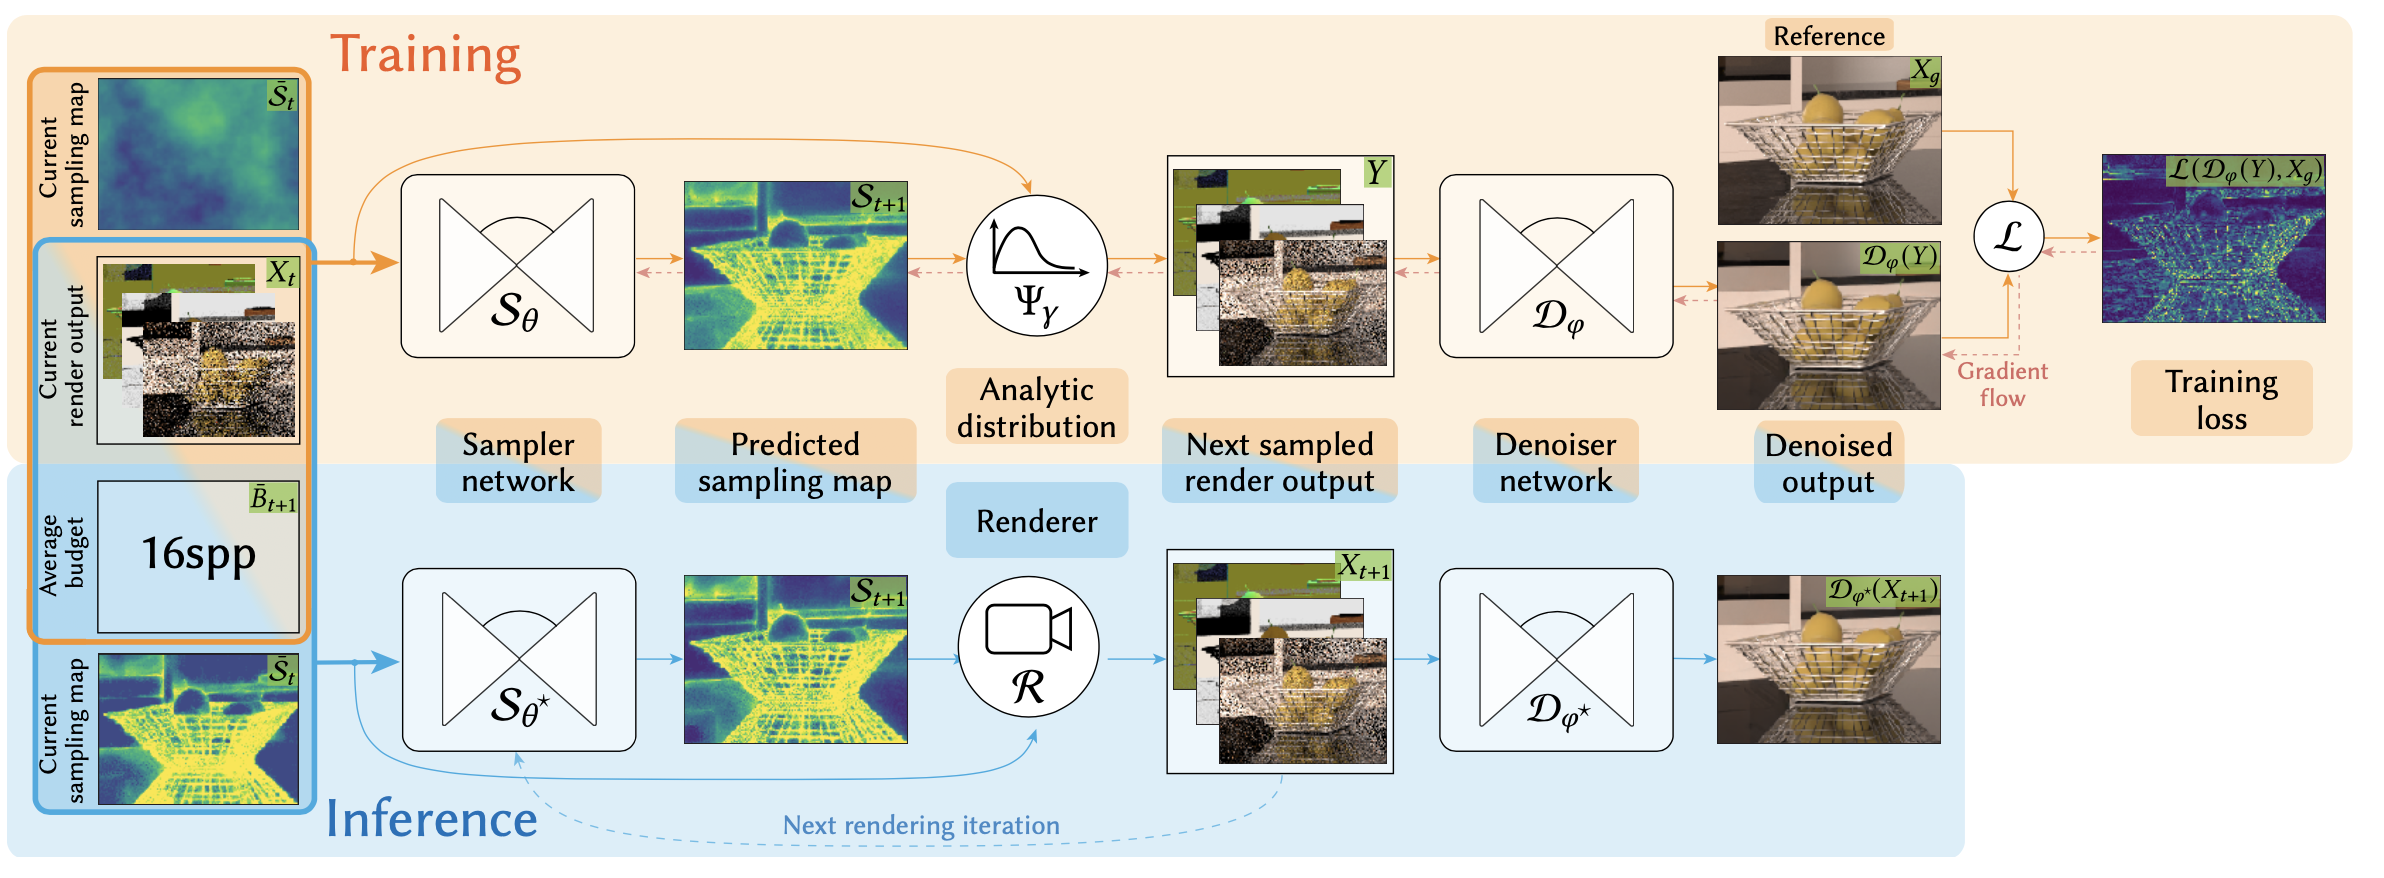
\includegraphics[width=160mm]{image/pipeline.png}
\end{figure}

I will now brevly explain what are their fake renderer and how they work.

\par In DARS \cite{kuznetsov2018deep}, their fake renderer is $\R_{c}$ that renders 
new image by combining image from different numebr of samples per pixel. Using the fact that 
for uniformly independent sample, we have:
\[ \R(X,n+m) = \frac{n\R(X,n) + m\R(X,m)}{n+m} \]
Note that this is an equality on random variable. In other words, by taking two 
images $X_n$ and $X_m$ rendered with $n$ and $m$ samples 
respectively. We can combine them to produce an image $X_{n+m}$ that follows the same 
distribution as the image produced using $n+m$ samples.
So they  pre-render a set of images with power of two sample rates, $X_{2^0}$, $X_{2^1}$, \dots, $X_{2^k}$, 
where $2^k$ is a large number, they can produce an image of arbitrary sample count.
\begin{equation}
    \label{eq:3}
    \R_c(X,n) = \frac{\sum_{i=0}^k 2^i X_{2^i} g(n,i)}{n}
\end{equation}
where $g(n,i)$ is the binary value of the i-th lowest bit of $n$.

\par And more recently, \cite{10.1145/3550454.3555515} used a different fake 
  renderer $R_{a}$ that renders new images by generating
  new samples from a learned per pixel gamma function that has good properties. They proved
  that with a uniformly independent sample, we only need a second order 
  approximation of the renderer to make the gradient descend. So a well 
  chosen gamma function can be used to simulate a renderer. They chose a 
  gamma function according to the pixel distribution analysis done by 
  \cite{elek2019learning}.

\par And to derive those fake renderer, in \cite{kuznetsov2018deep} and
\cite{10.1145/3550454.3555515} they use a numerical derivation:
  \[ \frac{\partial \R(X,s)}{\partial s} = \frac{\R(X,s+h) - \R(X,s)}{h}\]
  But this simple numerical derivation is extremely noisy and thus makes the 
  training process unstable, so they suggest to average 
  it with a virtually large number of new renders with $s+h$ samples.
  \begin{align}
      \label{eq:4}
      \frac{\partial \R(X,s)}{\partial s} & = \E_h \left [\frac{\R(X,s+h) - \R(X,s)}{h} \right ] \\
      & = \frac{X_\infty - \R(X,s)}{s}
  \end{align}

\paragraph*{Perspective} Both of those fake renderer use the fake that the sample are
independant. Thus, they are not build to work with stratified sample. The question is
can we make a fake renderer where the optimisation still work that can take into account
that the real renderer use stratified sample. This is the problem on which I work 
on during the second part of my intership.

\section{Adaptive sampling using a prior knowledge on the repartition of the error}

In this section we don't use any denoiser.
We want to find a good sampling function $\Sm$ that minimise:
\[ \int_{I\in\Omega} \E \left [ \Los (\R(X, \Sm(X_n, B)), I_\infty) \right ] \]

\subsection{The idea}

My first idea take advantage of the fact that asymptotically, empirically, we have 
the following relationship for each pixel $p$ \cite{10.1145/237170.237265}:
\begin{equation}
    \label{eq:99}
    e_p = \frac{b_p}{n_p^{a_p}}
\end{equation}
where $e_p$ is the square $\ell_2$ error, $n_p$ is the number of samples, 
and $a_p$, $b_p$ are two parameters that depend on the function we are 
integrating and the random sequence we are using. With our formalism 
\ref{eq:1}, with a linear loss on each pixel (the loss is the sum of 
the losses on each pixel), we have:
\[ \Los(\R(X,n)_p) = \frac{b_p}{n_p^{a_p}} \]
with $n$ by $\Sm(X_m, B)$. Now we have a formulation that is no longer 
dependent on the renderer.

\paragraph*{Remark} With a random independent samples, we know that $b_p = Var(f)$ and 
$a_p=1$. But we are interested in the case where we use stratified samples.

Here is an example of what the map $a$ and $b$ look like on a scene:
\begin{figure}[H]
    \centering
    \caption{Parameter $a$ and $b$}
    \label{fig:a}
    \begin{tabular}{ccc}
    \includegraphics[width=45mm]{image/without/gt.png}
    & 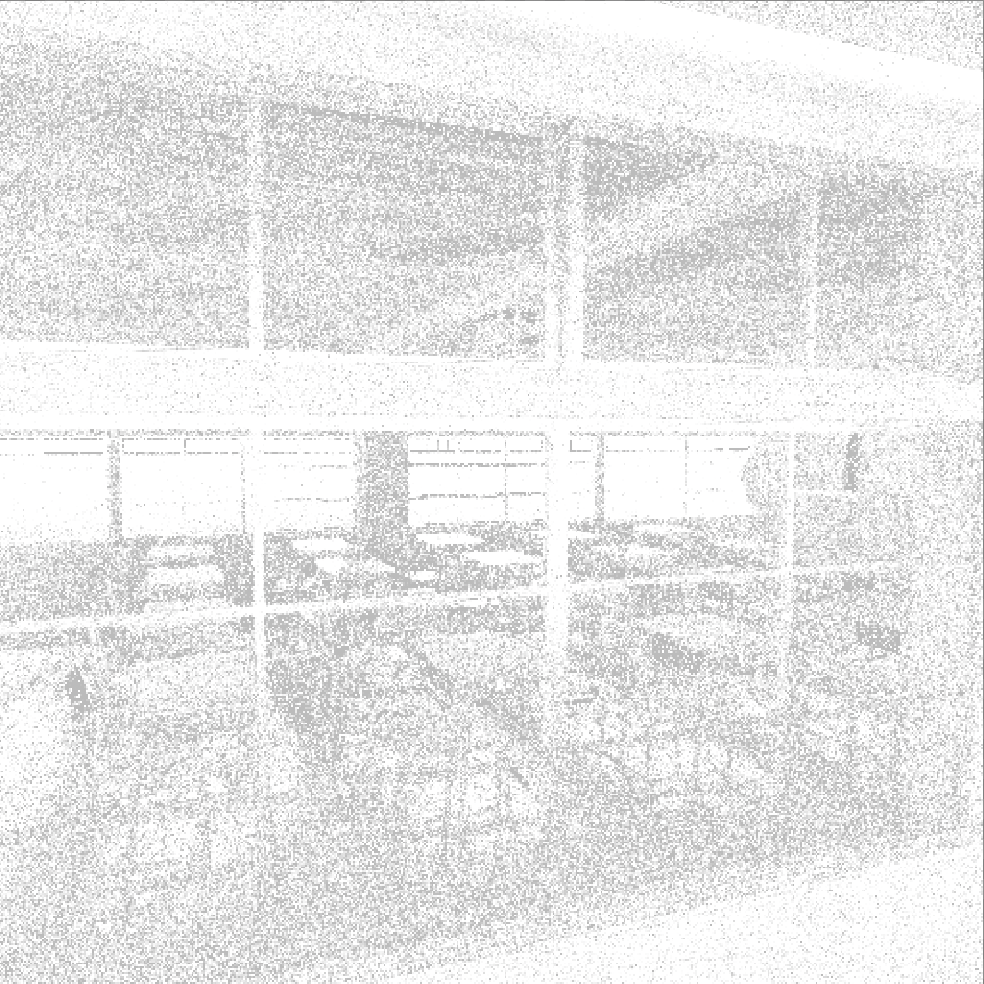
\includegraphics[width=45mm]{image/without/a.png}
    & 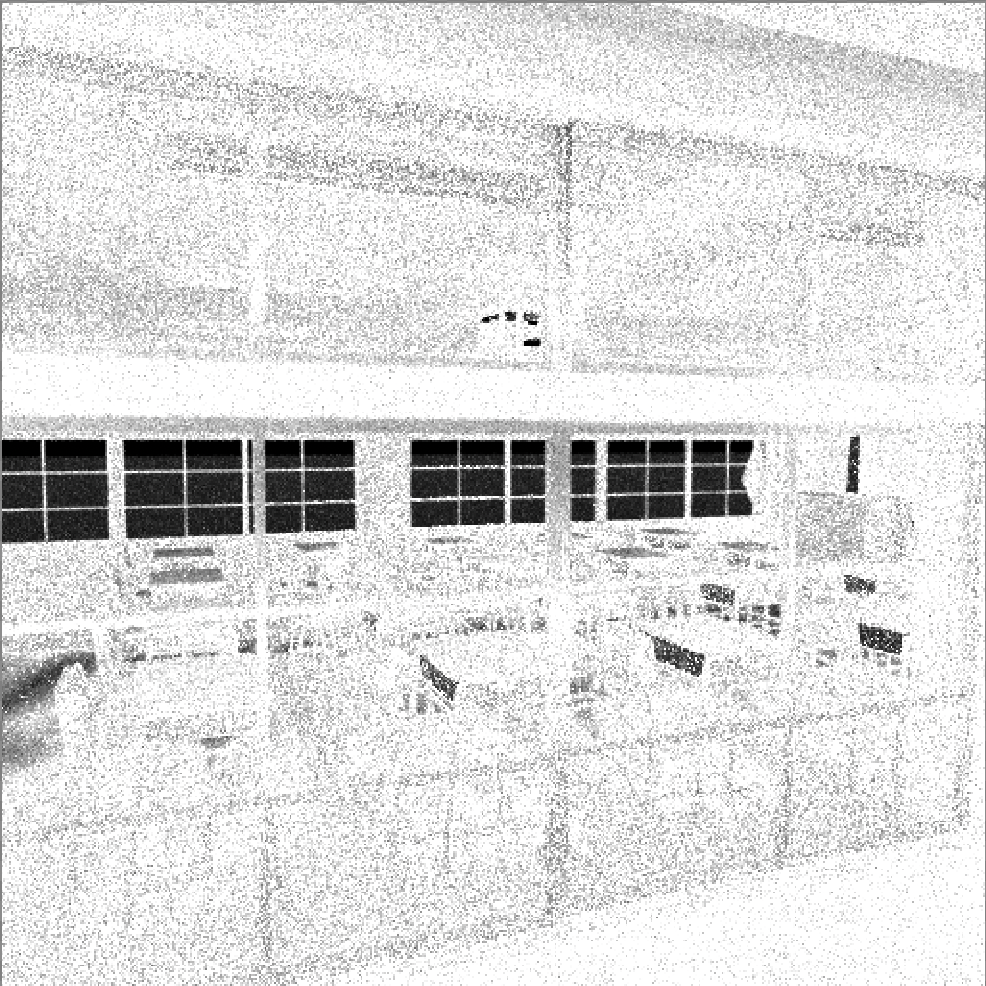
\includegraphics[width=45mm]{image/without/b.png} \\
    scene & a & b
    \end{tabular}
\end{figure}

If we have the parameter $a$ and $b$ of the equation \ref{eq:99} for each pixel, 
we can do different type of sampling function. Two examples are given in 
the next subsection.


\subsubsection{Minimal error expectation}
\paragraph*{Goal} The goal, is to have a sampling function $\Sm_{min}$ that produce
 an image with globally minimal error. That minimise the sum of error of each pixel.

\par By doing some optimisation, we can also use a straightforward algorithm 
to optimise the average error with $P$ being the total number 
of pixels. To do this, we introduce two functions:

\[ gain(p) = \frac{b_p}{(n_p+1)^{a_p}} - \frac{b_p}{n_p^{a_p}} 
\qquad loss(p) = \frac{b_p}{(n_p-1)^{a_p}} - \frac{b_p}{n_p^{a_p}} \]

where $gain(p)$ is the error gain by adding a sample in pixel $p$ 
(it is a negative value), and similarly $loss(p)$ is the error loss
 by deleting a sample in pixel $p$ (it is a positive value). We now 
 have the following property:
\paragraph*{Small Lemma} \textit{If we have a sampling map $n$, 
and two pixels $p$ and $p'$ such that 
\[gain(p) + loss(p') > 0\] 
we can get a better sampling map by swapping a sample from $p'$ to $p$.}\\ 
With this little lemma, we can derive an algorithm to minimise the 
average error as long as we observe point $p$ and $p'$ with positive 
gain by swapping a sample between the two. Here is a quick Python 
program that does this.

\begin{lstlisting}[language=Python, caption=Equal Error]
def minimalErrorAverage(a,b,N):
    n = N/P

    for step in range(512):
        eGain = b*(1/(n+1).pow(a) - 1/n.pow(a)) 
        eLoss = b*torch.where(n > 1, (1/(n-1).pow(a) - 1/n.pow(a)), 1e9)

        eGainSorted, Gainindices = ePlus.sort()
        eLossSorted, Lossindices = eMinus.sort()

        n[Gainindices[:P/2]] += 1  
        n[Lossindices[:P/2]] -= 1
    
    e = (b/n.pow(a)).mean()
    return (e,n) \end{lstlisting}

The result of this algo is this sample map:
\begin{figure}[H]
    \centering
    \caption{Sampling map and the corresponding error of $\Sm_{min}$}
    \begin{tabular}{ccc}
    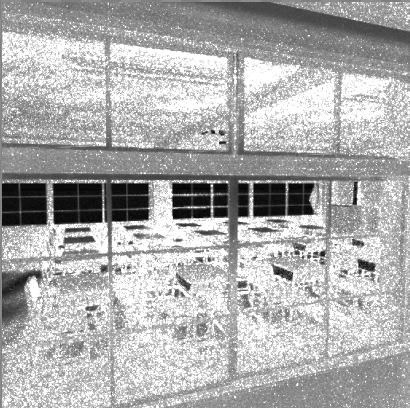
\includegraphics[width=45mm]{image/without/sm_min.png}
    & 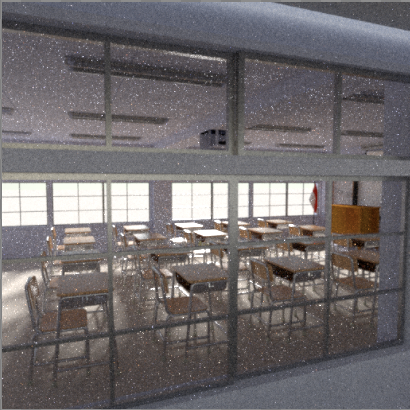
\includegraphics[width=45mm]{image/without/normal_min.png}
    & 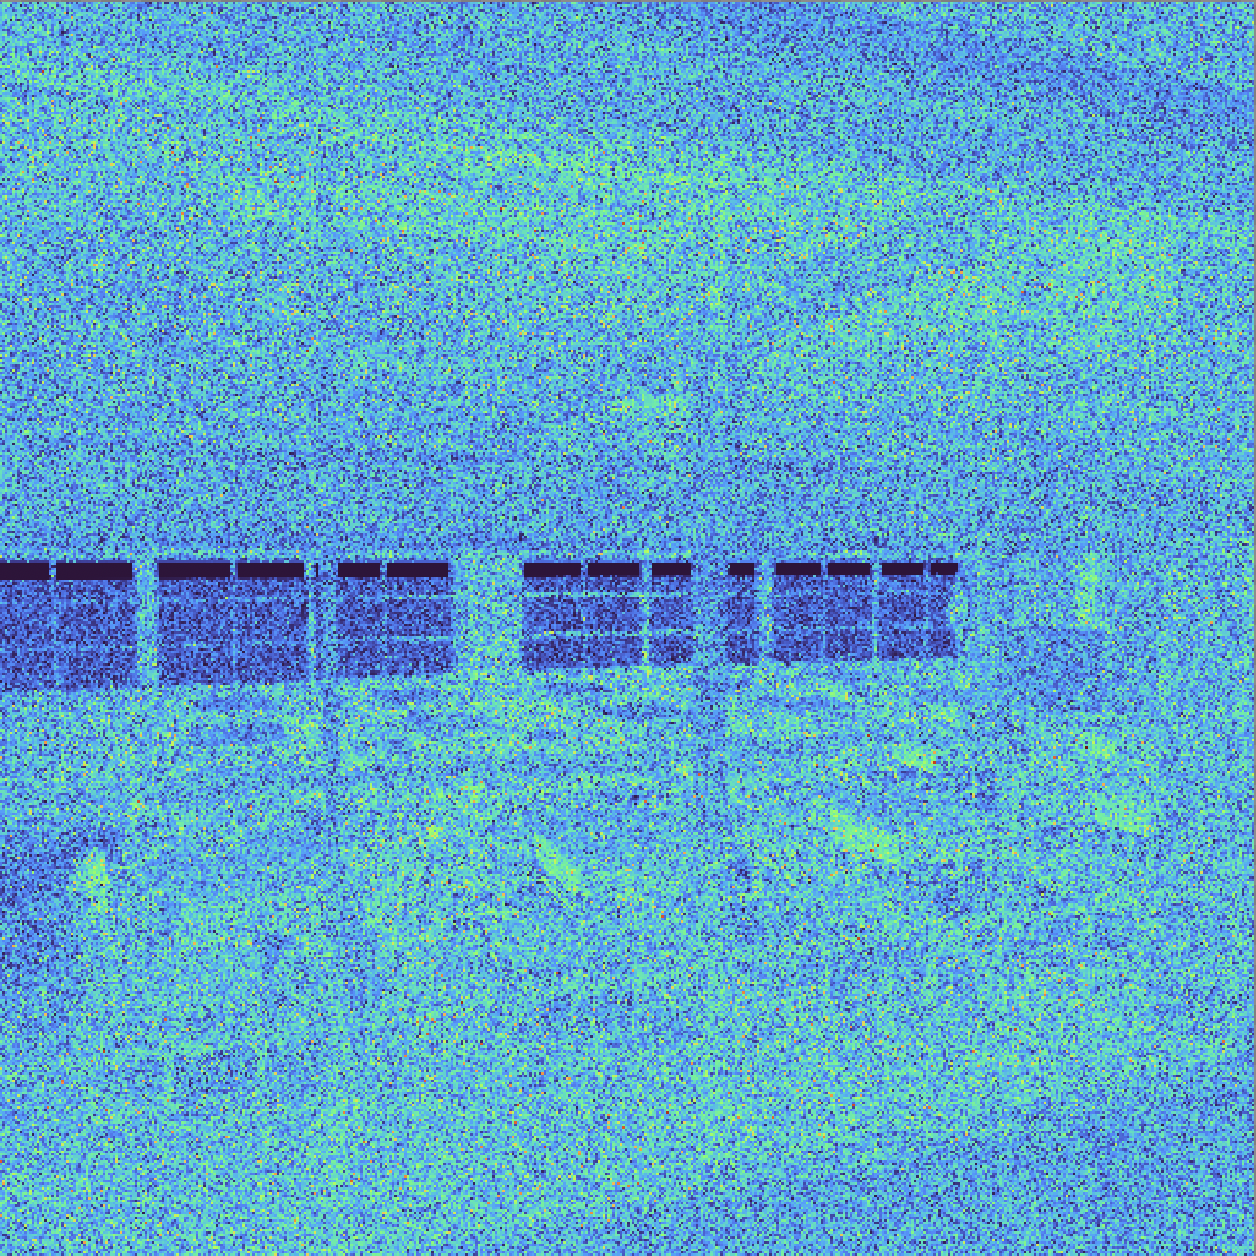
\includegraphics[width=45mm]{image/without/RMSE_min.png} \\
    sampling map & image & RMSE error
    \end{tabular}
\end{figure}

\subsubsection{Equal error expectation}

\paragraph*{Goal} We may want to do other things that just minimising the global error, 
like having a sampling function $\Sm_{equal}$ 
that produce an image where each pixel integration as the same expectation of error. 

\par To do so, by reversing the equation, from an error level $e$, we can get the number 
of samples needed to have that expected error for each pixel:
\[ n_p(e) = (b_p/e)^{1/a_p} \]
So, if we set a budget $B = \sum_p n_p$, we can perform a dichotomy 
on this function to adjust the error level $e$ to have $B$ samples 
globally. Here is the function in Python with pytorch that gives the appropriate 
error level $e$ and a sample map $n$ such that $B = \sum_p n_p$.
\begin{lstlisting}[language=Python, caption=Equal Error]
def equalErrorSamplingFunction(a, b, N):
    maxE = 1e-8
    minE = 1e5

    maxN = (b / maxE).pow(1./a).sum()
    minN = (b / minE).pow(1./a).sum()

    while(abs(maxN - minN) > 0.001):
        e = (maxE + minE)/2
        mn = (b / e).pow(1./a).sum()
        if (mn > N):
            maxE = e
        else:
            minE = e

        maxN = (b / maxE).pow(1./a).sum()
        minN = (b / minE).pow(1./a).sum()

    e = (maxE + minE)/2
    n = (b / maxE).pow(1./a)
    return (e,n) \end{lstlisting}

Thus, in practice, with accurate $a$ and $b$ parameters, 
we can produce an image with this error distribution with 
an average budget of 64 samples per pixel:

\begin{figure}[H]
    \centering
    \caption{Sampling map and the corresponding error of $\Sm_{equal}$}
    \begin{tabular}{ccc}
    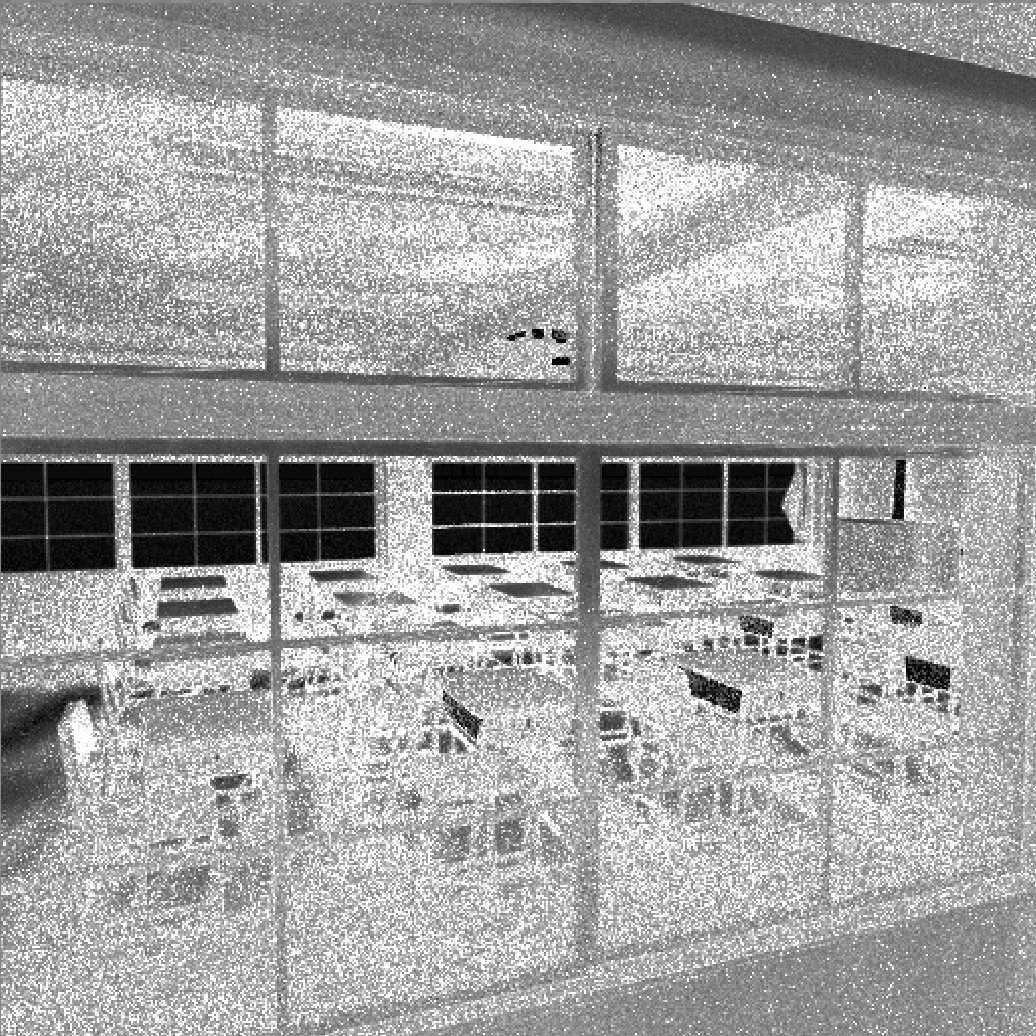
\includegraphics[width=45mm]{image/without/sm.png}
    & 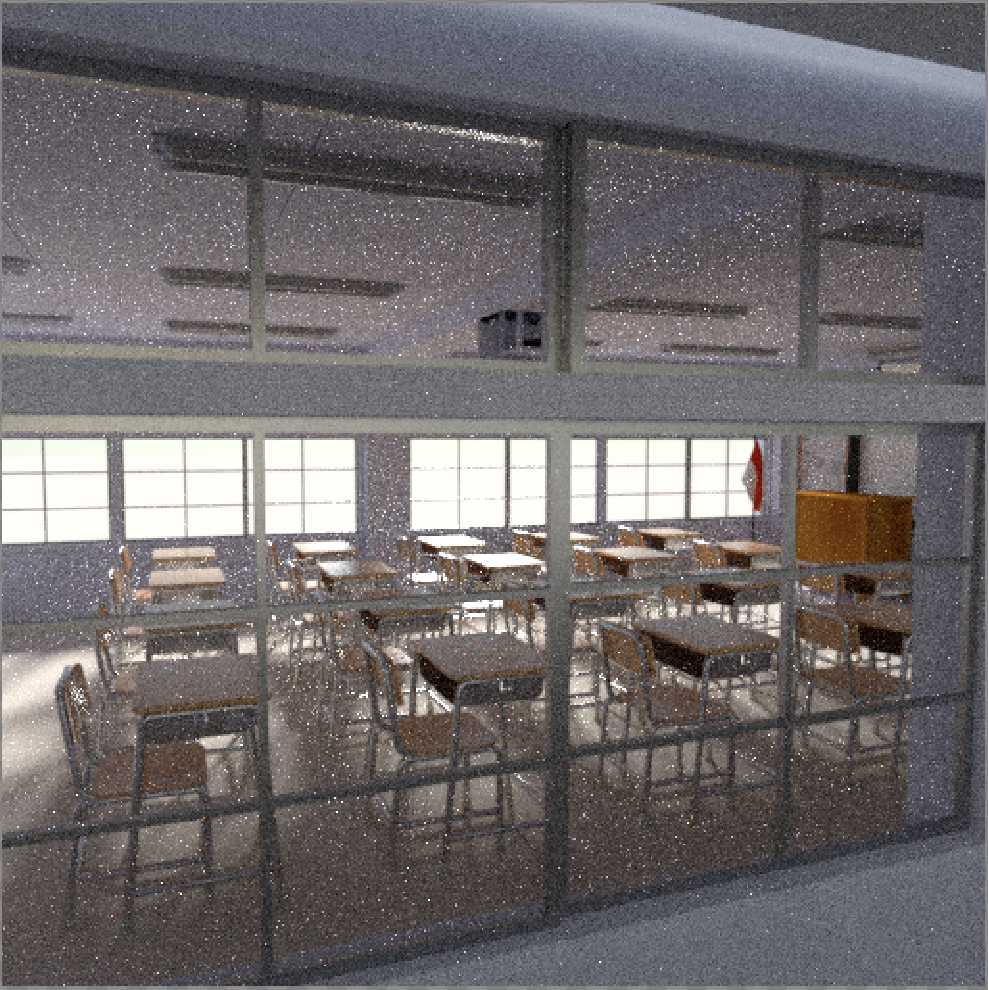
\includegraphics[width=45mm]{image/without/normal.png}
    & 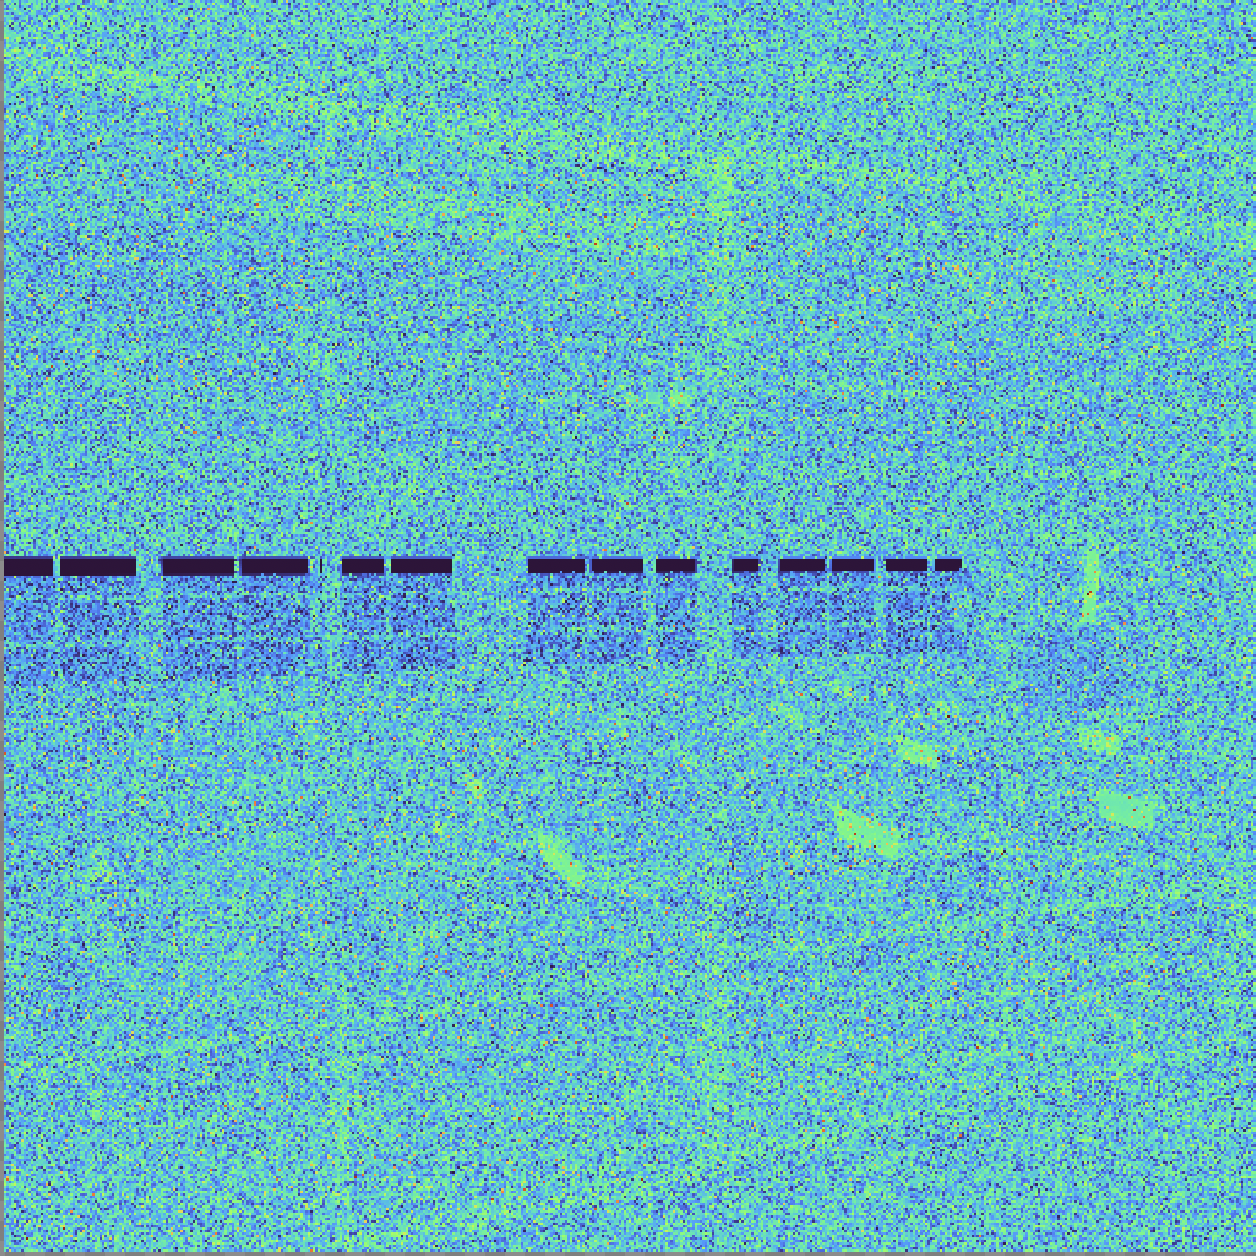
\includegraphics[width=45mm]{image/without/RMSE_mean.png} \\
    sampling map & image & RMSE error
    \end{tabular}
\end{figure}

It is still not perfect. The problem we had, as discussed later, is that it 
is really hard to estimate these parameters $a$ and $b$ accurately. It need 
a huge computational power.

\subsubsection{Theoretical Error comparaison}

Because it's fun, we can make a side by side comparison of the error map for a scene of 
two sampling function $\Sm_{min}(X), \Sm_{equal}(X)$ with the error map
of the default sampling function $\Sm_{uni}(X)$ that always output $\bar m$.

\begin{figure}[H]
    \centering
    \caption{Comparaison of the error, after using different sampling function}
    \begin{tabular}{ccc}
    $\Sm_{min}(X)$ & $\Sm_{uni}(X)$ & $\Sm_{equal}(X)$ \\
    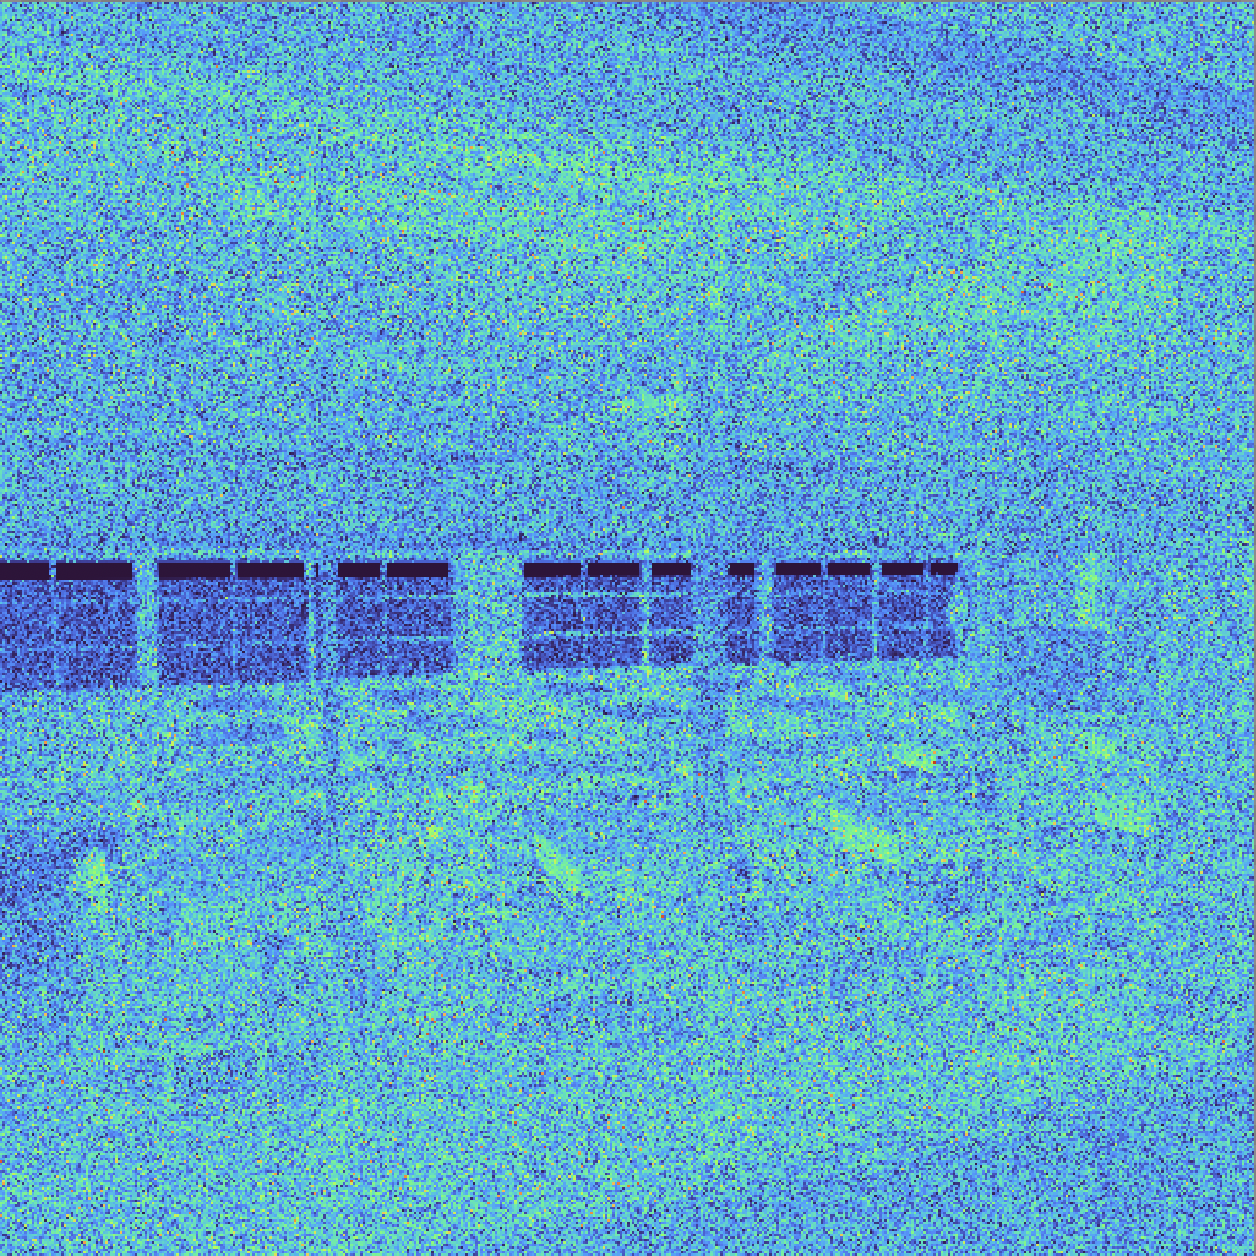
\includegraphics[width=45mm]{image/without/RMSE_min.png}
    & 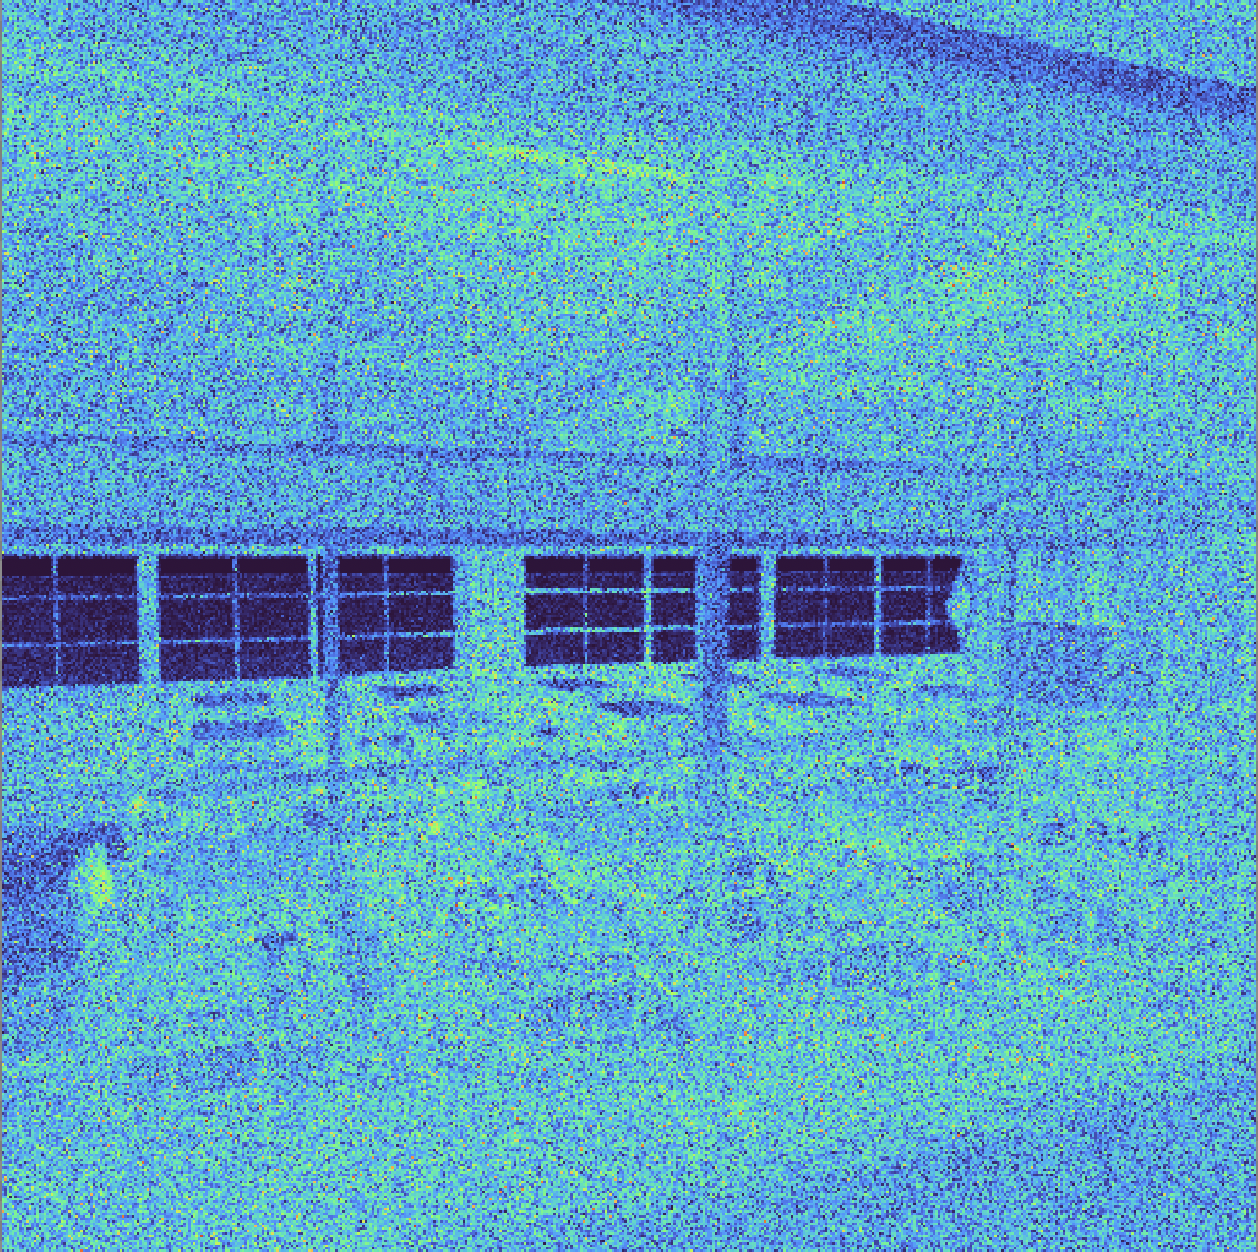
\includegraphics[width=45mm]{image/without/RMSE_uni.png}
    & 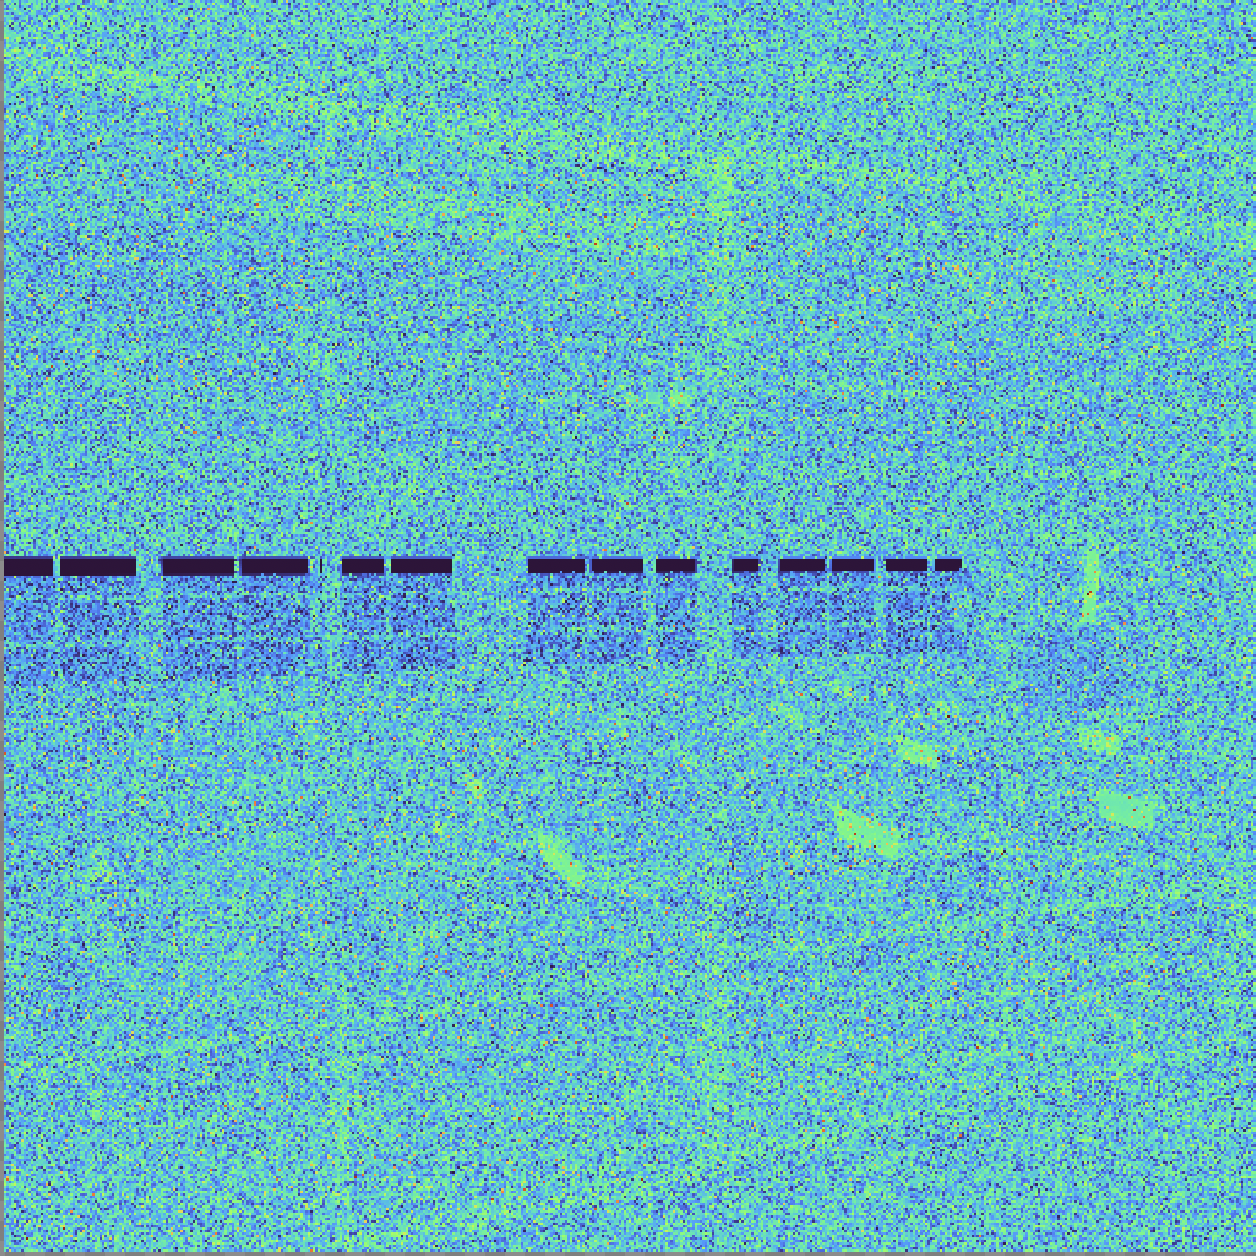
\includegraphics[width=45mm]{image/without/RMSE_mean.png} \\
    RMSE=$0.195$ & RMSE=$0.196$ & RMSE=$0.252$
    \end{tabular}
\end{figure}
As you can see, the error with $\Sm_{min}$ isn't much smaller than 
the error in the default sampling function $\Sm_{uni}$.
 And to get a uniform error, we lose a global quality. 
\par This gives us a general insight: \textit{uniform error
 and minimising mean error require two sampling maps that 
 are really different}. In other words, to minimise the 
 average error, you don't want to have the same error in 
 every pixel.

\subsection{Prediction of the parameter $a$ and $b$}

After reading the previous section, you may wonder how we get 
  the parameter $a$ and $b$. The plan is simple. Can we predict 
  these parameters with a minimum number of information that is 
  fast to compute. 
  In pratice, what we did is the following:
  Given the rendering image with $1$, $2$, $4$ 
  spp, is it possible to find a good enough approximation 
  of $a$ and $b$ thanks to a neural network?

\par The plan is simple, from a dataset taht contains for many scene $X$ pairs: 
(input=$X_{\bar m}$,output=$(a,b)$) with a small $m$, train a 
convolutional neural network that from $X_{\bar m}$ output $a$ and $b$.

\paragraph*{Discussion} The idea is simple, but there 
is a big problem, it is probably not true that we can find a 
strong enough link between image with low sample ($X_{\bar m}$) 
to their respective convergence rate ($a$ and $b$). We clearly have a 
huge lack of information. Our hope is that, as in rendering, neighbours 
pixel integrale are similare, the network has more information 
that just the $m$ samples of the pixel to predict $a$ and $b$. This 
is the reason why we use a CNN for the network, to maximise the chance
to find a link between neighbours pixel.

\subsubsection{Create a dataset}

\par The first difficulty was creating a dataset to train the network on. 

Our model is really simple, as input to our network we have 
the image with low sample count $X_{\bar m}$, and as output we have the 
two parameter maps $a$ and $b$. So all we had to do was find 
the truth parameters $a$ and $b$ for each scene.

\par To do this, for each scene, for each power of two 
($2^p$) up to 2048, I had generated $20$ images with $2^p$ 
samples per pixel. Then I averaged the error at each sample count. 
And finally, I did a linear regression in log space to find the 
parameter, as we can rewrite the equation
\ref{eq:99}:
\[ \log(e_p) = -a_p\times \log(n_p) + \log(b_p)\]
Below is the result of the regression for a typical pixel of an image
\begin{figure}[H]
    \centering
    \caption{Linear regression of the error in function of the number of sample}
    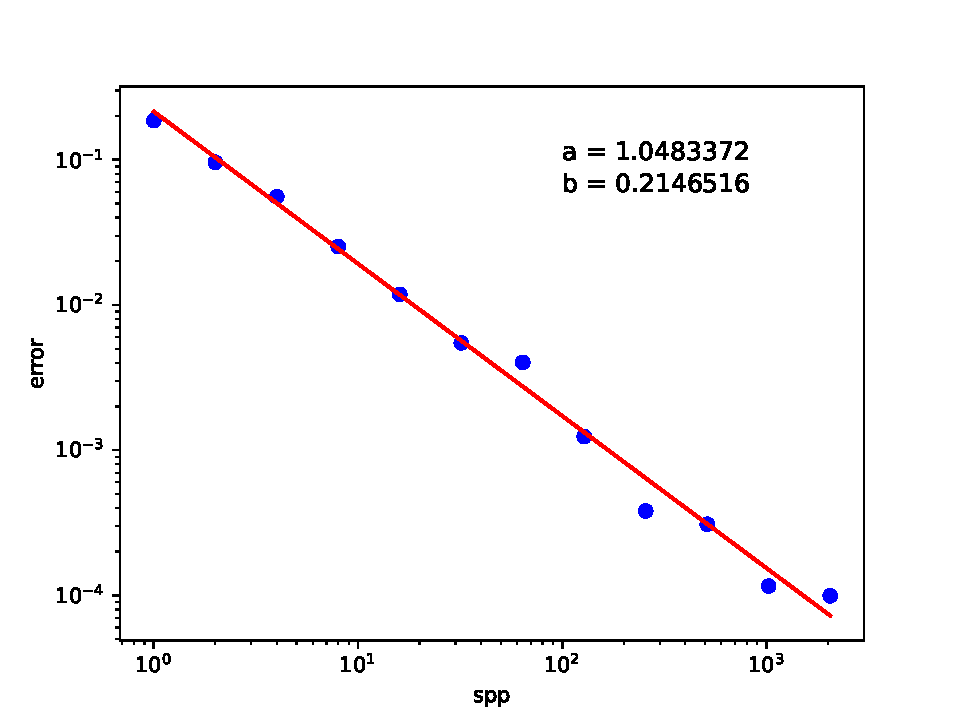
\includegraphics[width=70mm]{image/without/plotsobol.pdf}
\end{figure}
As you can see, the regression points are quite noisy. So our 
ground truth isn't noise free. But we didn't have the 
computational resources to compute more images to get a 
noise-free ground truth, as you can see in the figure \ref{fig:a}.
\par I said that it's noisy because we have to remember that this graphic is in log scale.
So even a small $\epsilon$ error in $a$, can result in a exponential error when predicting 
the error of integration. 

\par In the end, we generated the ground truth from 200 scenes of size 512x512.
I have generate for 150 Go of render, it took more than a week on a 32 CPU core. 
And the final size of the dataset is less than a 1Go, it only contains $a$ and $b$ for each scene. 
With more hindsight, we should have generate smaller image, maybe 64x64, but with higher quality
(more realisation per sample count).

\subsubsection{Implementation details}

\paragraph*{Network} We used the same architecture of UNET as in \cite{kuznetsov2018deep}. For more clarity, 
here is below the schema of the network. The schema has be taken from the article 
\cite{kuznetsov2018deep}.
\begin{figure}[H]
    \centering
    \caption{Schema of the network from \cite{kuznetsov2018deep}}
    \begin{tabular}{c}
    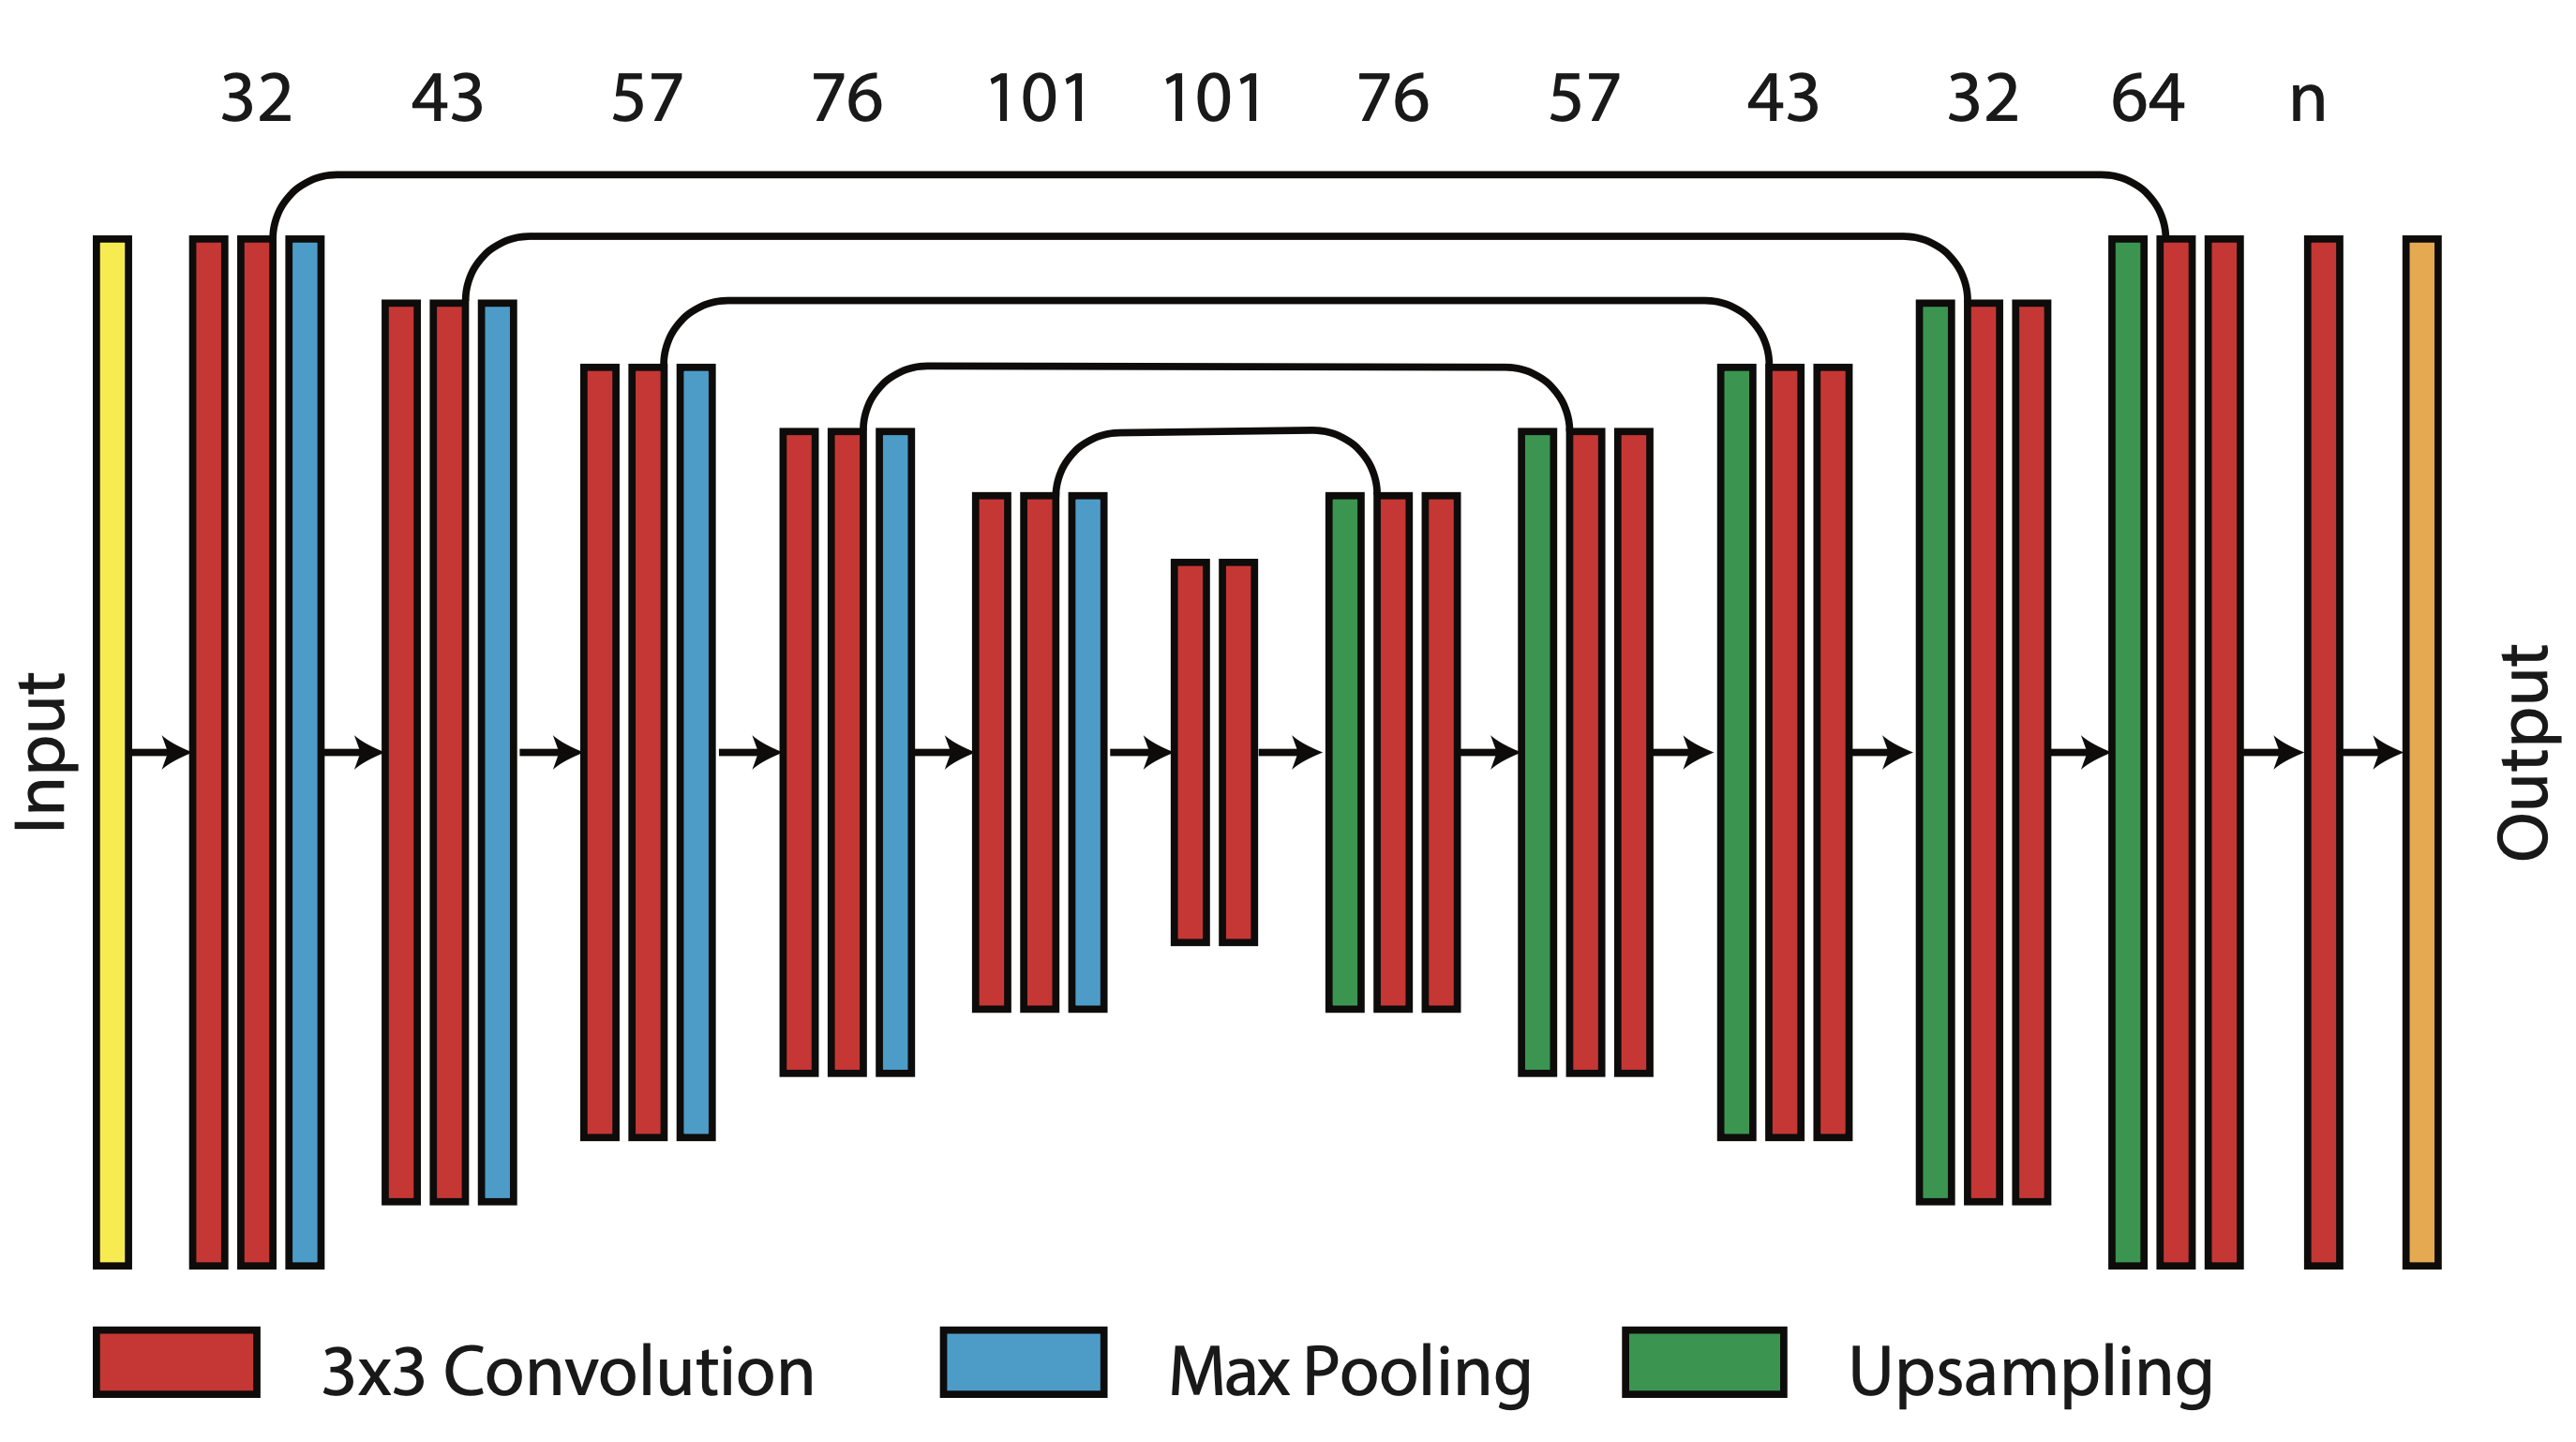
\includegraphics[width=120mm]{image/network.png}
    \end{tabular}
\end{figure}
In our case, $n=2$ as we predict 2 channels for $a$ and $b$. The input of the network
is:
\begin{itemize}
    \item The images $X_{\bar 1}$, $X_{\bar 2}$ and $X_{\bar 4}$, to give the network the starting point 
    of the progression of convergence.
    \item Some auxiliarys buffers, like the normal map, the depth map and the albedo map, to help the 
    network to link neighbours that should be similare.
\end{itemize}

We trained it with the Adam optimiser \cite{kingma2017adam} 
with $\epsilon=10^{-4}$ and the loss $\ell_2$.

\subsubsection{Result}

Here is an example of the prediction we got:
\begin{figure}[H]
    \centering
    \caption{Predicted parameter $a$ and $b$ for the classroom scene}
    \begin{tabular}{cccc}
    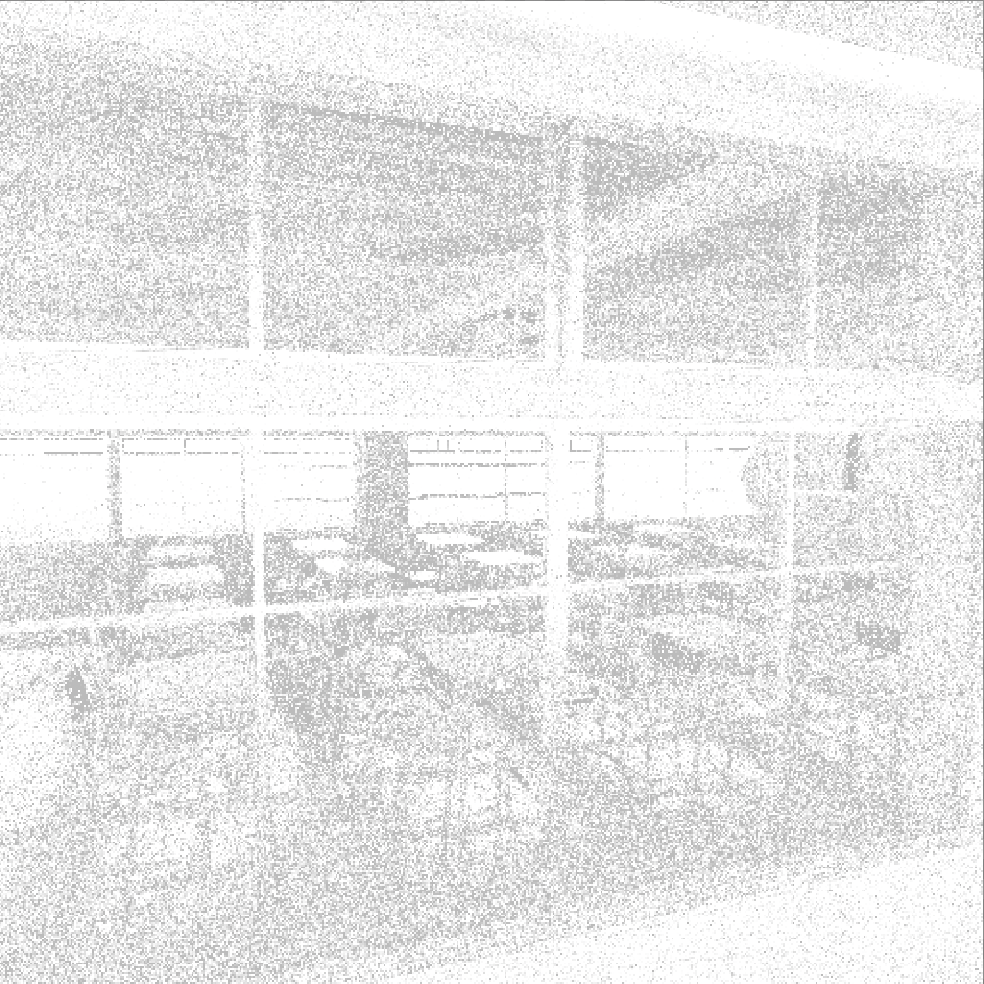
\includegraphics[width=35mm]{image/without/a.png}
    & 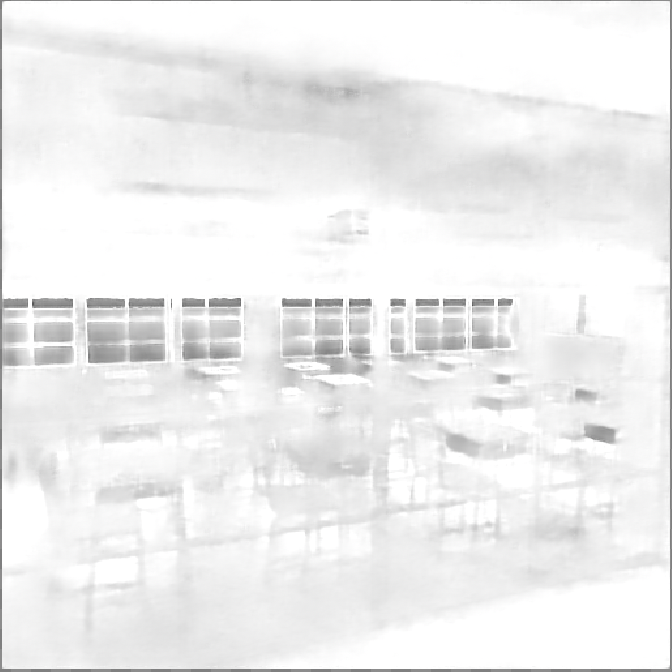
\includegraphics[width=35mm]{image/without/pa.png}
    & 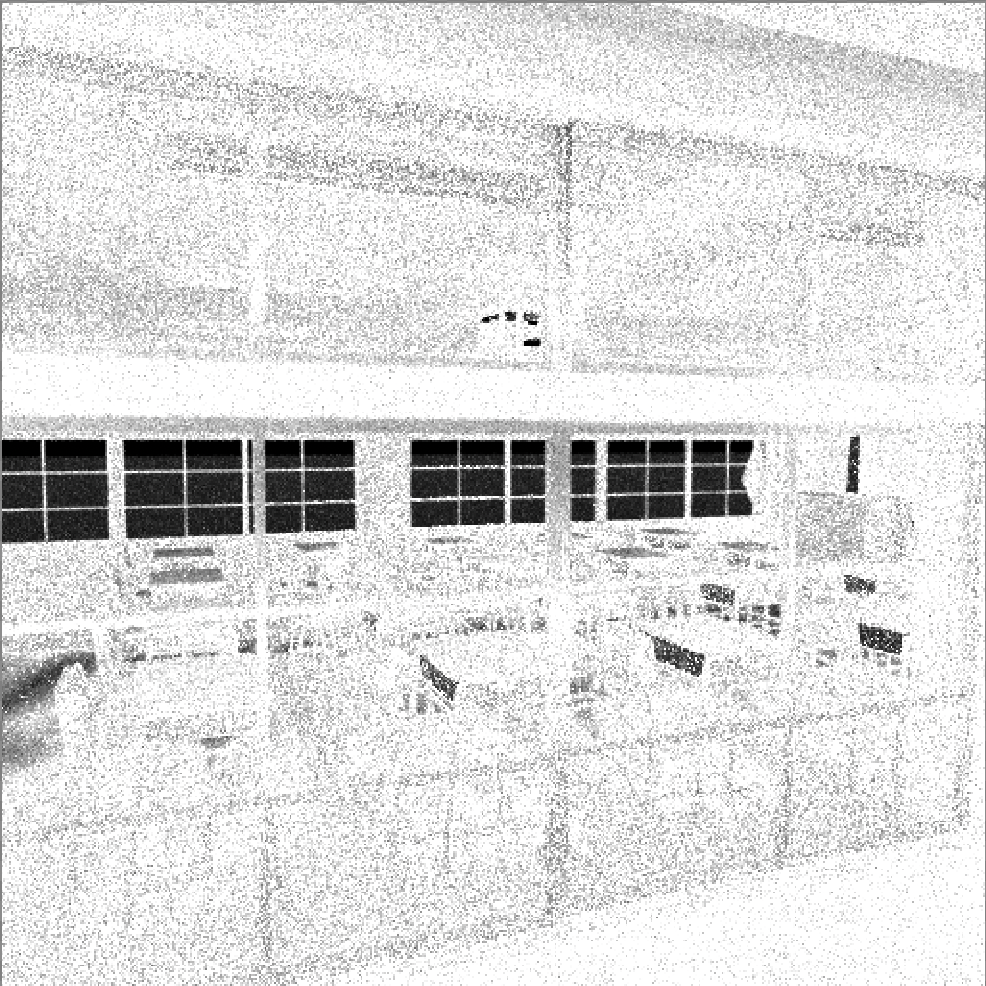
\includegraphics[width=35mm]{image/without/b.png}
    & 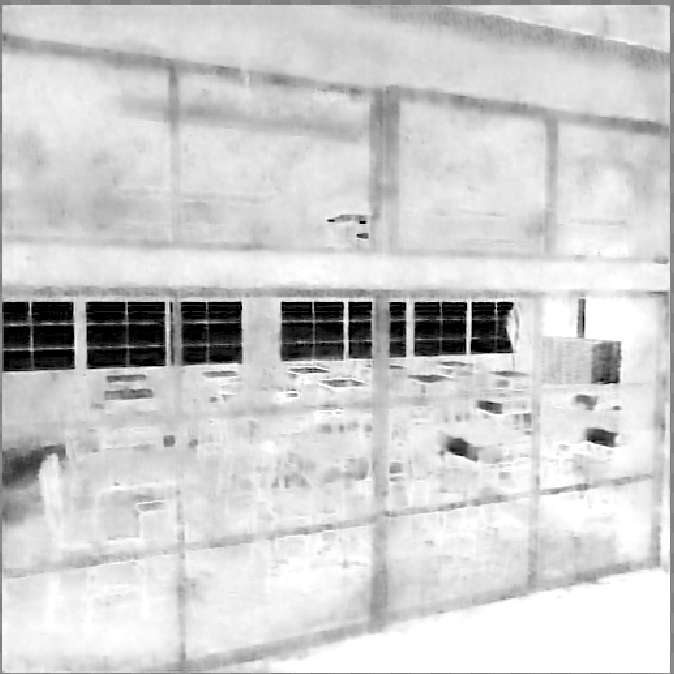
\includegraphics[width=35mm]{image/without/pb.png} \\
    groundtruth a & predicted a
    &groundtruth b & predicted b \\
    \end{tabular}
\end{figure}
And here what append when I use these prediction of $a$ and $b$ with the sampling
function $\Sm_{min}$.
\begin{figure}[H]
    \centering
    \caption{Comparaison of $\Sm_{min}$ using the prediction of $a$ and $b$, with $\Sm_{uni}$}
    \begin{tabular}{|c|c|c|c|}
        \hline
        Scene & $\Sm_{min}$ & $\Sm_{min}$ error & $\Sm_{uni}$ error\\
        \hline
        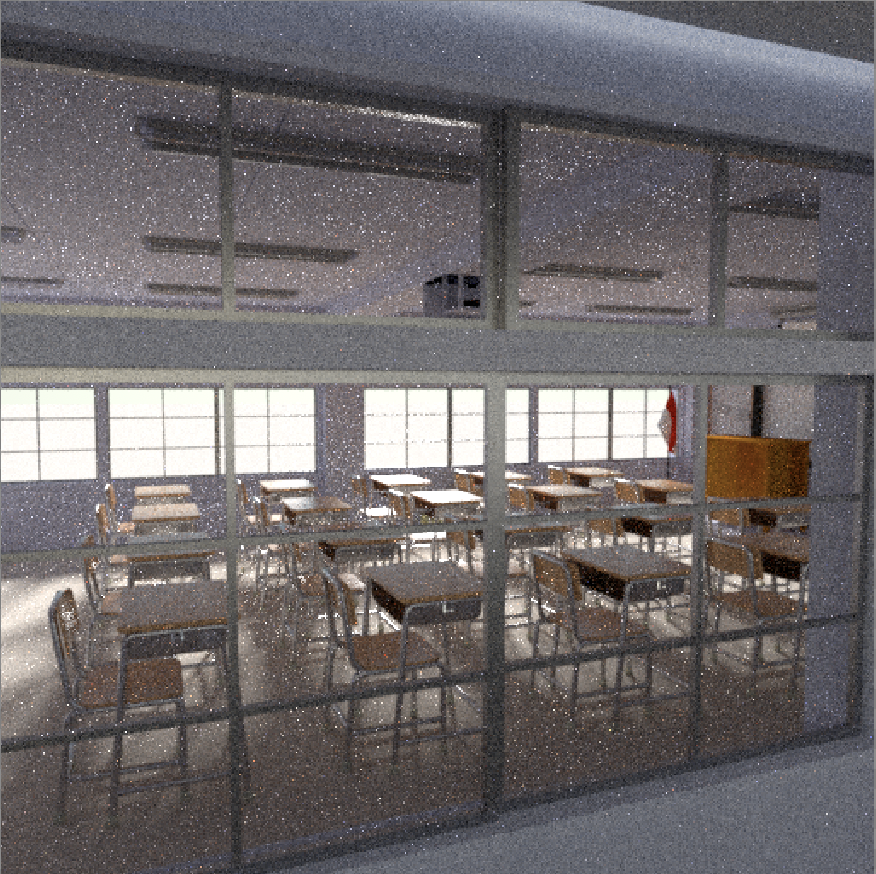
\includegraphics[width=35mm]{image/without/pimage.png}
        & 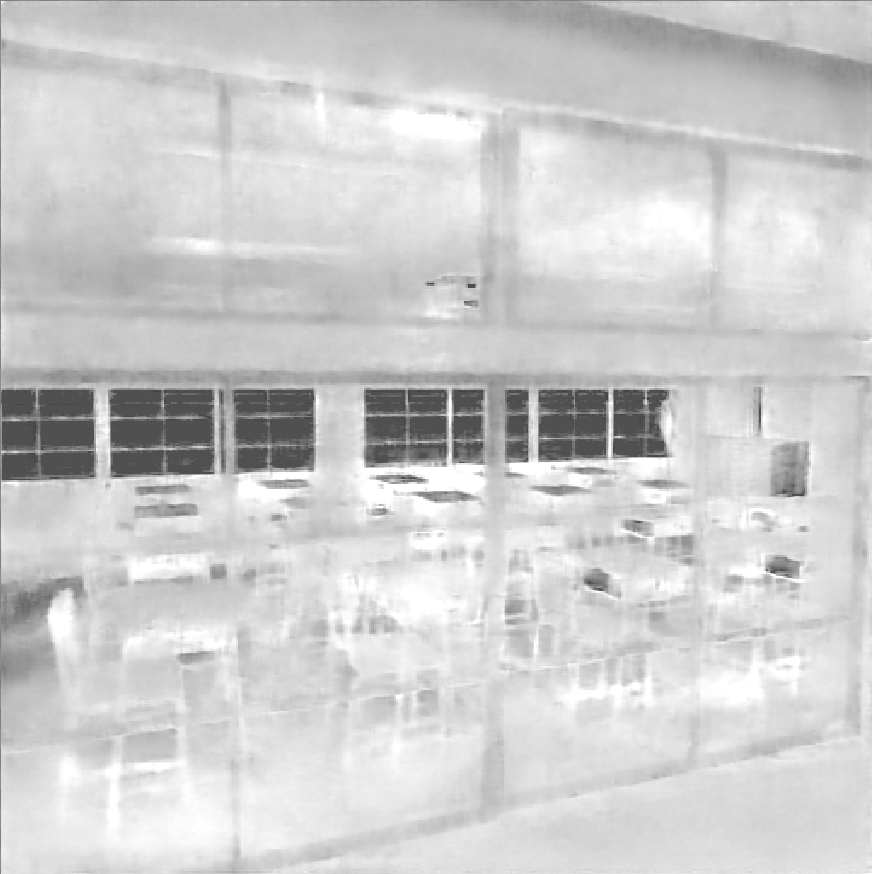
\includegraphics[width=35mm]{image/without/psm.png}
        & 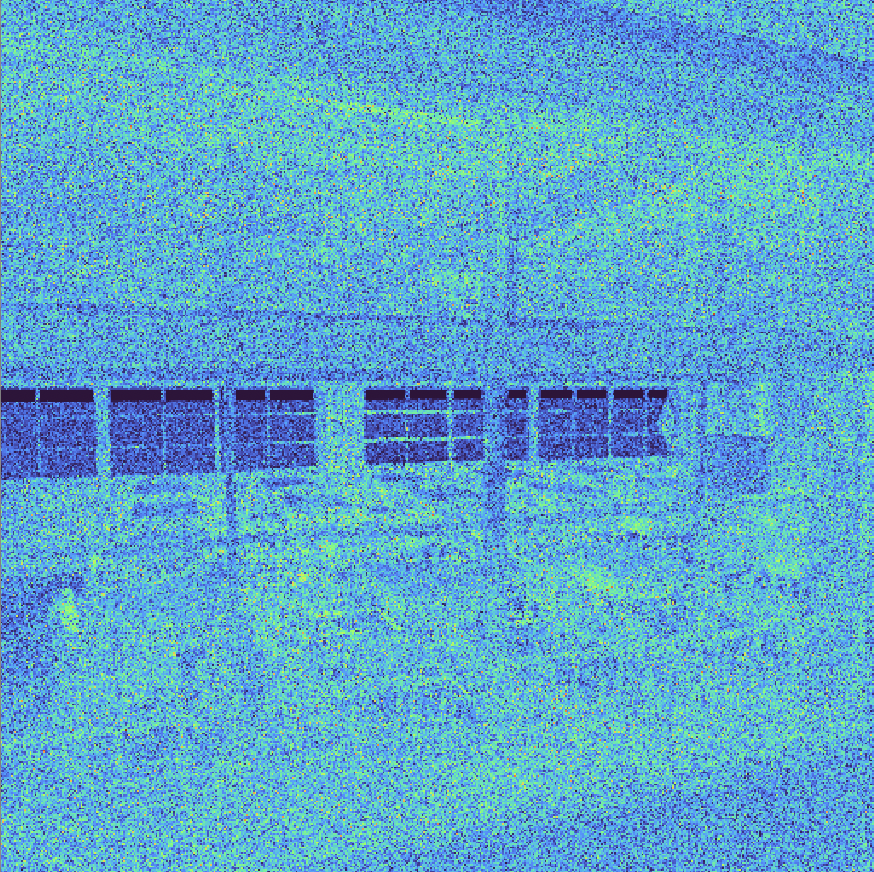
\includegraphics[width=35mm]{image/without/perror.png}
        & 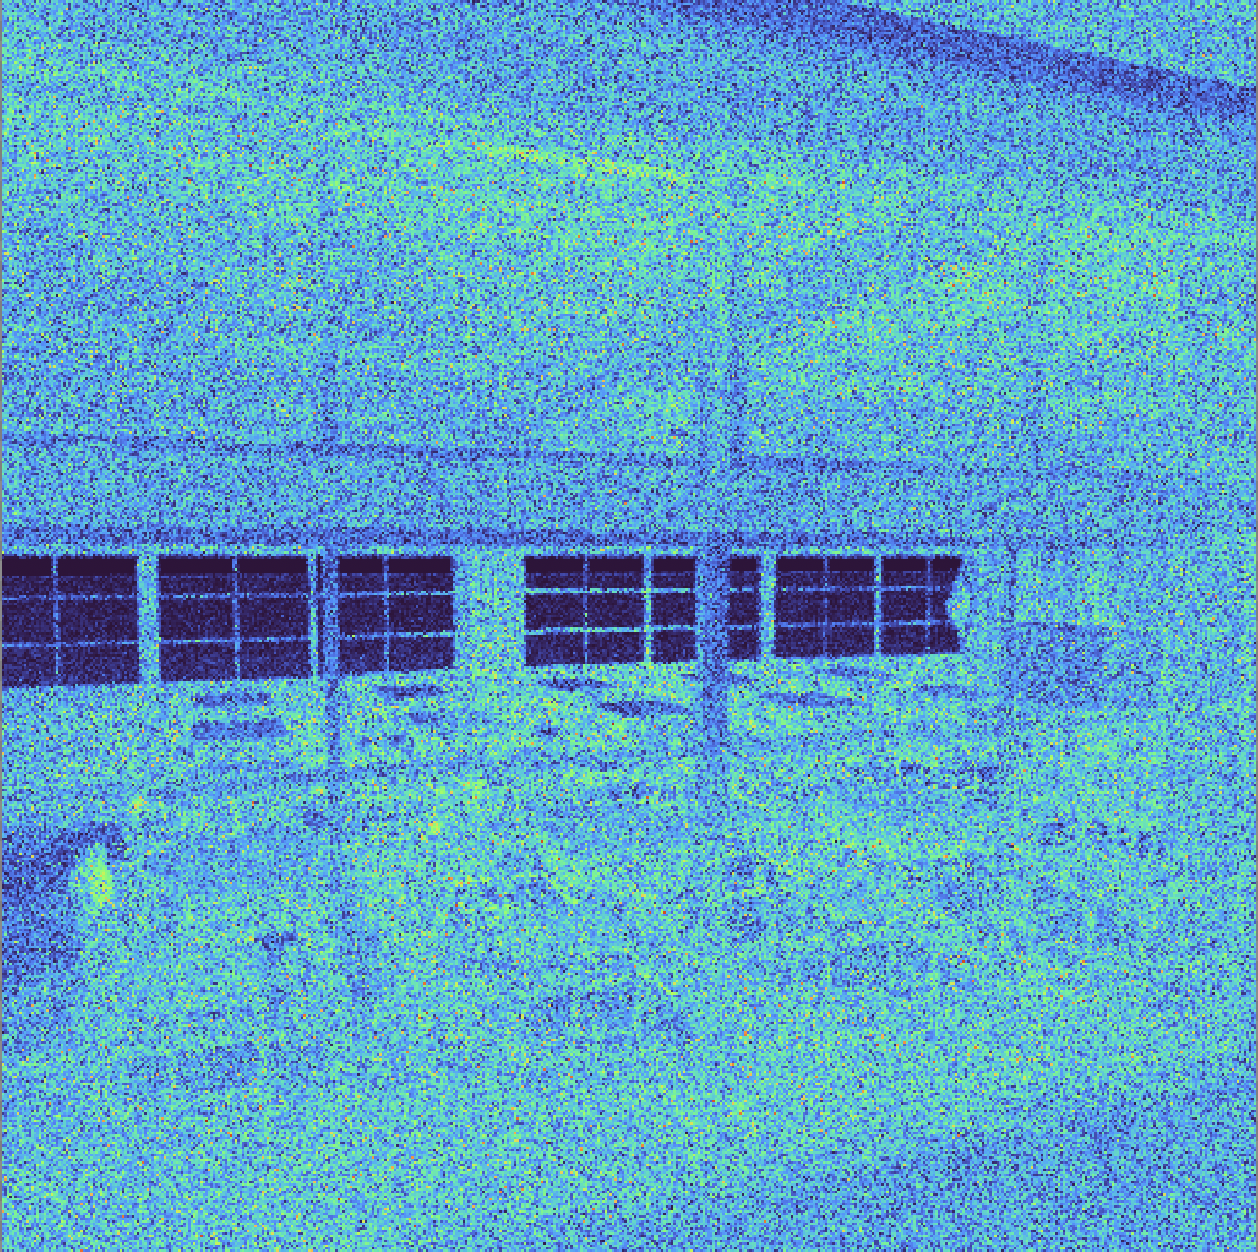
\includegraphics[width=35mm]{image/without/RMSE_uni.png} \\
         &  & RMSE=0.193 & RMSE=0.196 \\
        \hline
        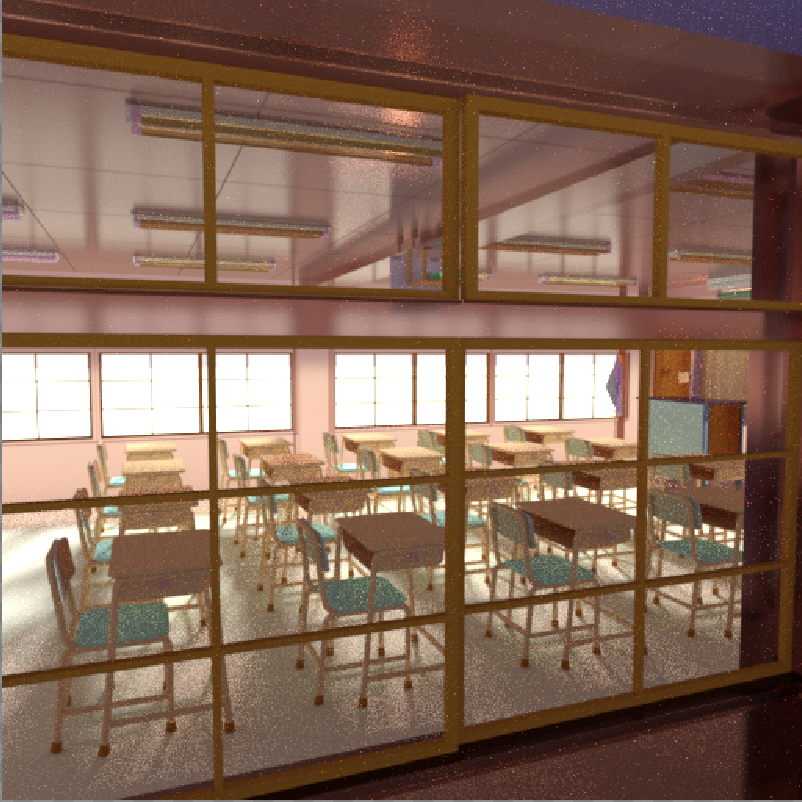
\includegraphics[width=35mm]{image/without/ppgt.png}
        & 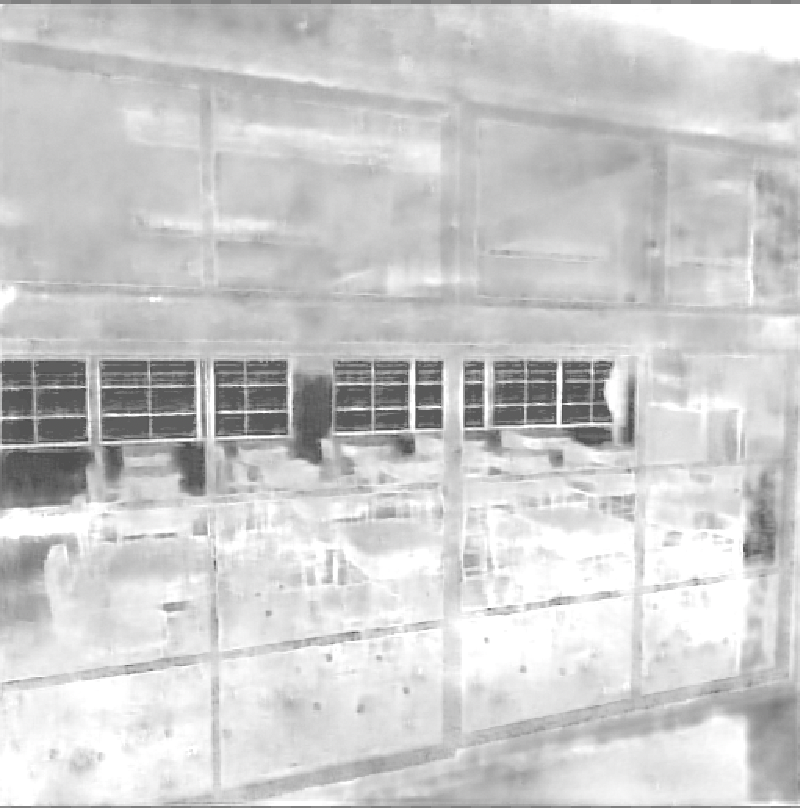
\includegraphics[width=35mm]{image/without/ppsm.png}
        & 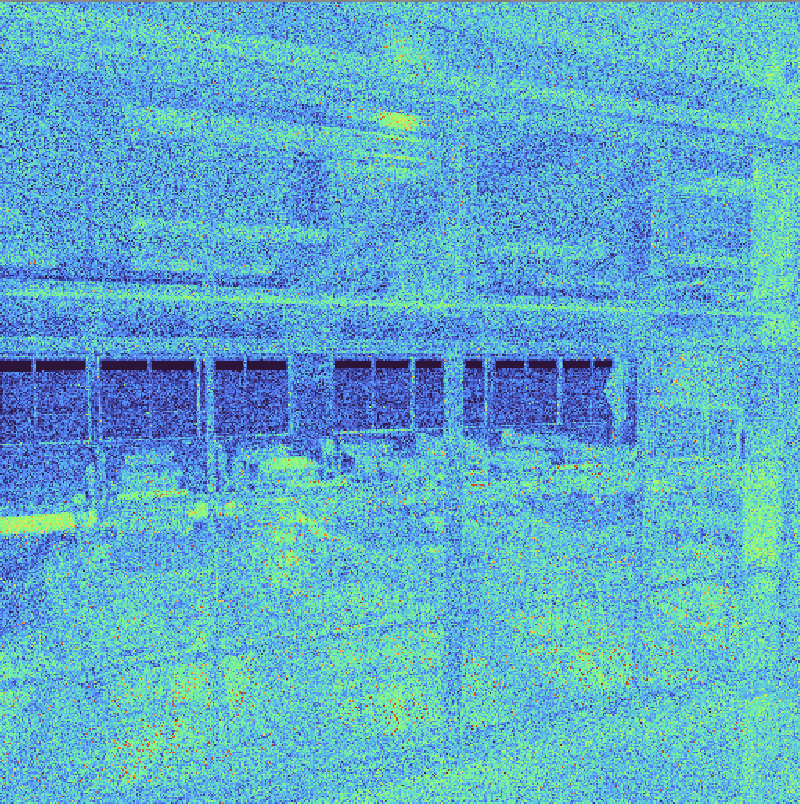
\includegraphics[width=35mm]{image/without/ppp.png}
        & 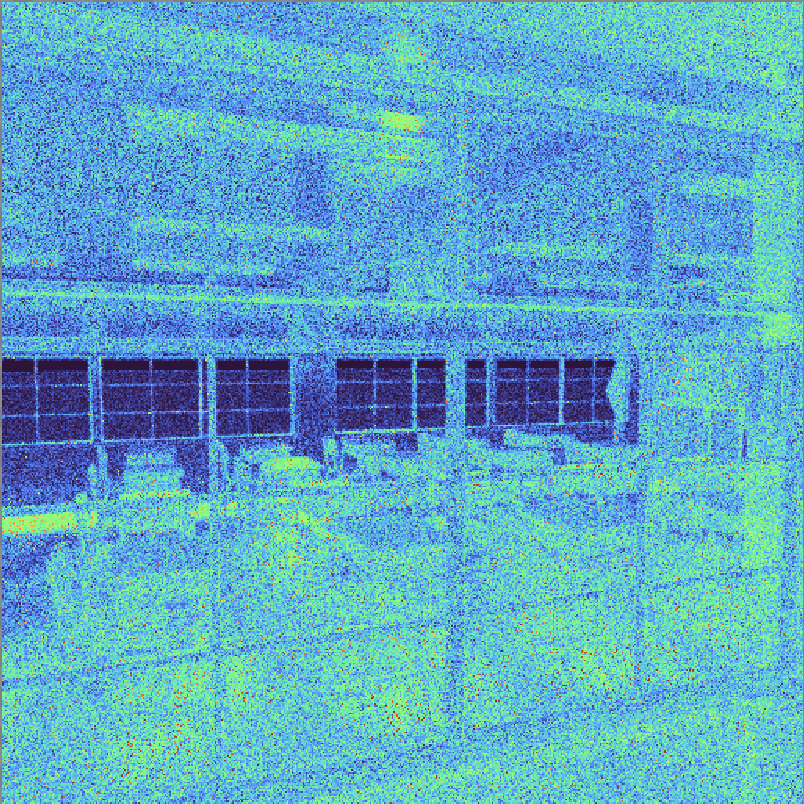
\includegraphics[width=35mm]{image/without/pp_norm.png} \\
         &  & RMSE=0.257 & RMSE=0.252 \\
        \hline
    \end{tabular}
\end{figure}
In the first scene we have a improvement in the error, but in the second scene, we do 
even worst than with the default sampling function $\Sm_{uni}$. To summarize, our
prediction of $a$ and $b$ combined with out $\Sm_{min}$ doesn't always reduce 
the error.

\paragraph*{Discussion} We haven't managed to make this idea fully work, 
 but the idea is promising. Maybe with more data we could get a better result. 
 Or maybe, with an image with low number of sample, we probably don't have 
 enough information to deduce the parameter $a$ and $b$, and we can't get 
 something any better even with more training. 

\paragraph*{Perspective} To continue this section, we could have try to increass
the size of the dataset, or improve the quality of our groundtruth $a$ and $b$, by maybe 
a better regression algorithm. Or maybe try a different neural network architecture.

\par This conclude the first part of my work during the intership.


\section{Adaptive sampling by direct optimisation}

The goal of this section is to find a fake renderer that is designed to work
with stratified samples. But before describing our fake renderer, let's first look at
some properties of stratified sample when we use them in adaptative sampling.

\subsection{Analysis on adaptive sampling with stratified samples}

We will note $\R(X, h | s)$ the rendering image of the scene X, using $h$ sample of
a sequence that has already used $s$ sample.

\par A nice property of the independent sample is that for each $X,s,h$ we have
\[ \E_h[\R(X,h | s)] = X_\infty \]
In other words, when we add new samples, the expectation of the image 
with these new samples is the ground truth. This simple property no 
longer holds when we have a stratified sample.
\par Let's look at an example in two dimensions with a fully stratified 
sequence, like the one in \cite{10.2312:sr.20211287}. Suppose we already 
have a know where where our first samples are in blue, the news samples 
are in red.

\begin{center}
    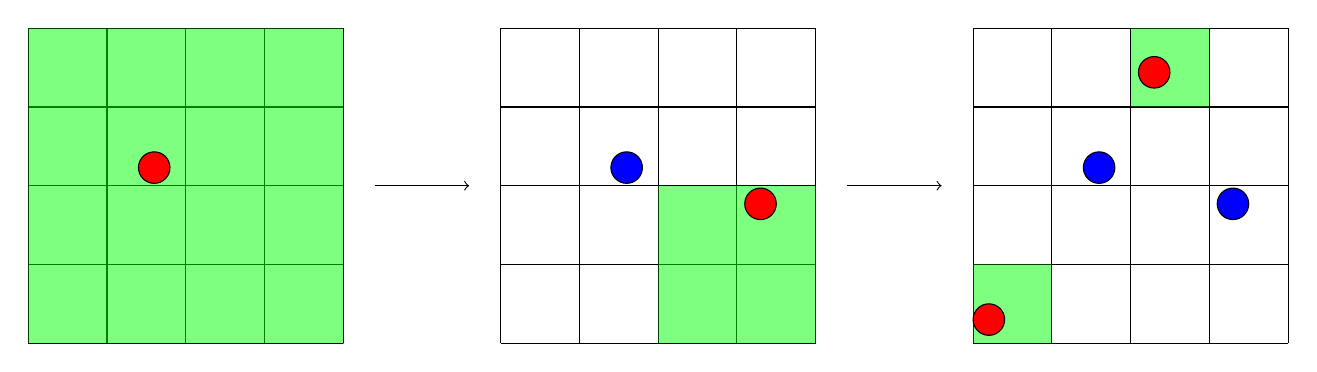
\begin{tikzpicture}
        \draw (0,0) grid (4,4);
        \draw [fill=green, opacity=0.5] (0,0) rectangle (4,4);
        \draw [fill=red] (1.6,2.23) circle (0.2);

        \draw [->] (4.4,2) -- (5.6,2);

        \draw (6,0) grid (10,4);
        \draw [fill=blue] (7.6,2.23) circle (0.2);
        \draw [fill=green, opacity=0.5] (8,0) rectangle (10,2);
        \draw [fill=red] (9.3,1.77) circle (0.2);

        \draw [->] (10.4,2) -- (11.6,2);

        \draw (12,0) grid (16,4);
        \draw [fill=blue] (13.6,2.23) circle (0.2);
        \draw [fill=blue] (15.3,1.77) circle (0.2);
        \draw [fill=green, opacity=0.5] (12,0) rectangle (13,1);
        \draw [fill=green, opacity=0.5] (14,3) rectangle (15,4);
        \draw [fill=red] (12.2,0.3) circle (0.2);
        \draw [fill=red] (14.3,3.44) circle (0.2);
    
    \end{tikzpicture}
\end{center}
The green part shows where the next sample can be. And as our sampler is stratified,
with the knowledge of where was our first sample, we know that the second sample can only
be in a quarter of the domain. That's why the expectation of this realisation is not the
the groundtruth, but only the true integrale of the corresponding quarter of the image.
\par This is just a consequences of the correlation between sample in stratified sample.

\par With this in mind, we can see that the analysis done by \cite{10.1145/3550454.3555515}
isn't really possible with stratified samples as it is already difficult to make an order 1 approximation of 
the distribution of next sample, it depends on the number of sample we already used. 
And as we are using sample in high dimension, we don't want to compute the exact green 
area where the next sample can be. Thus we can't know the true expectation of $\E_h[\R(X,h | s)]$.

\paragraph*{Discussion} The combination of images from different number of samples per pixel 
as done in \cite{kuznetsov2018deep} is not possible either. Thus, we needed to find a really 
different fake renderer in order to work with stratified samples.

\subsection{The derivation issue}

With stratified samples, we have another issue.
Let's take a closer look at the derivation of the equation \ref{eq:4}:
\begin{align*}
    \label{eq:4}
 \frac{\partial \R(X,s)}{\partial s} & = \E_h \left [\frac{\R(X,s+h) - \R(X,s)}{h} \right ] \\
    & = \E_h \left [\frac{(s\R(X,s) + h\R(X,h | s))/(s+h) - \R(X,s)}{h}\right ] \\
    & = \frac{\E_h \left [\R(X,h | s) \right ] - \R(X,s)}{s+h} \\
    & =\:???
\end{align*}
The issue we have, is that $\E_h \left [\R(X,h | s) \right ]$ not only is not $X_\infty$ 
but also depends on $h$. In pratice, we don't really know what is this expectation, so we
shouldn't really apply this technique to compute gradient.

\paragraph*{Confession of weakness} We know that we have this issue, but we haven't found 
a way to get a better final result, than with the approximation that 
$\E_h \left [\R(X,h | s) \right ] = X_\infty$. And this could be explained by the fact that 
even if this approximation is not true, the direction of the gradient is still good 
enough, and so the network converges in the good direction.

\subsection{Interpolation}

I can now introduce the fake renderer that we used, the only ways we found that can
take into account the fact that we used stratified sequence and not independent sample
is to generate images $X_{2^0}$, $X_{2^1}$, \dots, $X_{2^k}$, where $2^k$ is a large number
with the same sequence but with different sample count. And then interpolate for 
$n = 2^i + j$ ($j < 2^i$):
\begin{equation}
    \label{eq:5}
    \R_i(X,n) = \frac{2^i X_{2^i} + j X_{2^{i+1} | 2^i}}{n}
\end{equation}
where $X_{2^{i+1} | 2^i}$ is the image using $2^i$ samples of the sequence starting at 
$2^i$. The way to compute this from $X_{2^i}$ and $X_{2^{i+1}}$ is described in Appendix \ref{combi}.

\paragraph*{Discussion} This interpolation has many flaws, but it seems to be 
 the best way to approximation of the true renderer, that take into 
 account the fact that our samples are stratified. We have 
 $\E[R_i(X,n)] \approx \E[R(X,n)]$ and $\V[R_i(X,n)] \approx \V[R(X,n)]$.

\subsection{Implementation Details}

In this section, I discuss the implementation details needed to reproduce 
our results. I trained two networks, one for the denoiser and one 
for the sampler.

\paragraph*{Network details} I used two simple UNET for the sampler and the denoiser, 
it is the same architecture ad in the previous section and in \cite{kuznetsov2018deep}. 
The sampler outputs a single channel image representing the sampling map. And the denoiser
outputs a $13\times13$ channel image that represents a kernel of denoising as it 
is better than directly predicting the correct color in \cite{10.1145/3072959.3073708}. 
Here is an example of my denoiser:

\begin{figure}[H]
    \centering
    \begin{tabular}{cccc}
    \includegraphics[width=35mm]{image/denoiser/noisy.png}
    & \includegraphics[width=35mm]{image/denoiser/kernelmap.png}
    & \includegraphics[width=35mm]{image/denoiser/denoisy.png}
    & \includegraphics[width=35mm]{image/denoiser/gt.png} \\
    noisy (2 spp) & kernelmap & denoisy & groundtruth \\
    \end{tabular}
\end{figure}
A bigger image of this figure can be found in the annexe \ref{denoiserImage}:

\paragraph*{Dataset} I used 200 variations of scenes from \cite{resources16}, using 
the Tungsten renderer. I rendered at 256x256 resolution, with a ground 
truth of 65536 samples. For the input of our fake renderer, we also 
compute a cascade of images with power two samples per pixel using the 
same sequence.

\paragraph*{Training detail} I did the same thing as in \cite{kuznetsov2018deep}, since the range of color and albedo
is really large, I compress them by using a logarithm. $color -> \log(1+color)$. I chose to pass
as input of our network the color, albedo and the normal map with their respective variance. I also chose to 
pass the variance because, as suggested by classical methods without learning, the variance of 
the color is directly related to the error. In this way, the input 
of my network is close to what Bako has done in
\cite{10.1145/3072959.3073708}.
To summarize the entry of both of our network (denoiser and sampler) are:
\[x = (\log(1+color), \log(1+albedo), normal, \log(1+\V(color)), \log(1+\V(albedo)),  \V(normal)) \]
\begin{figure}[H]
    \centering
    \begin{tabular}{ccc}
    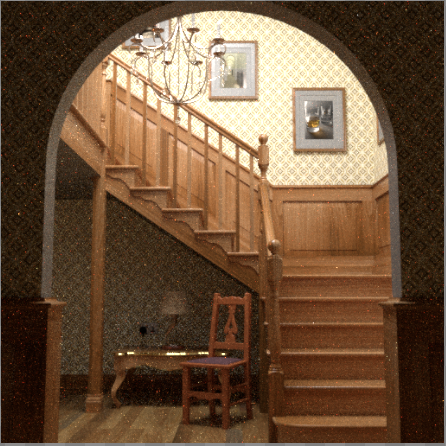
\includegraphics[width=45mm]{image/networkInput/color.png}
    & 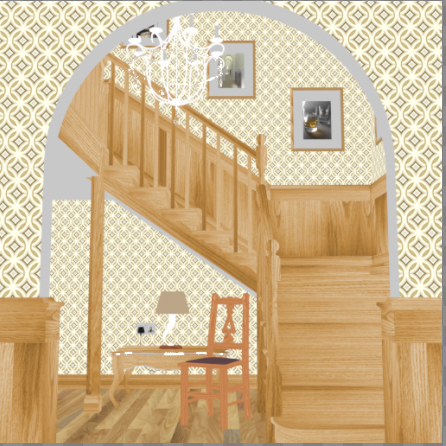
\includegraphics[width=45mm]{image/networkInput/albedo.png}
    & 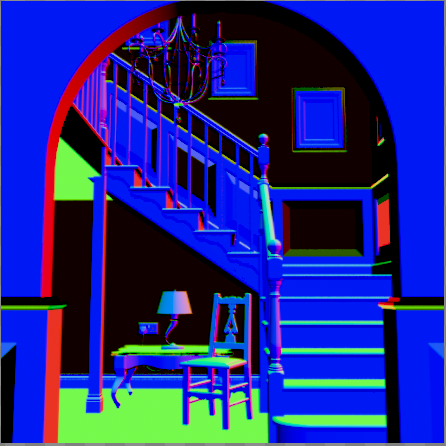
\includegraphics[width=45mm]{image/networkInput/normal.png} \\
    color & albedo & normal\\
\end{tabular}
\end{figure}
\begin{figure}[H]
    \centering
    \begin{tabular}{ccc}
    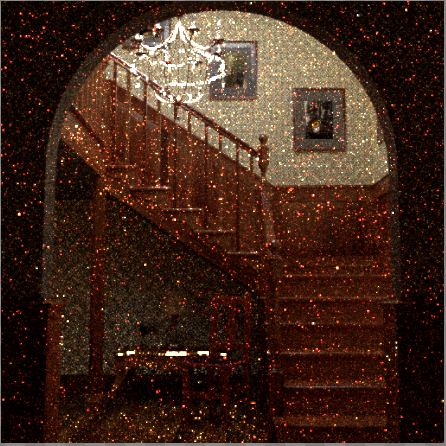
\includegraphics[width=45mm]{image/networkInput/colorV.png}
    & 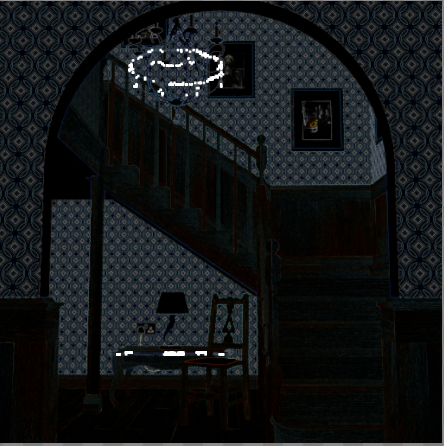
\includegraphics[width=45mm]{image/networkInput/albedoV.png}
    & 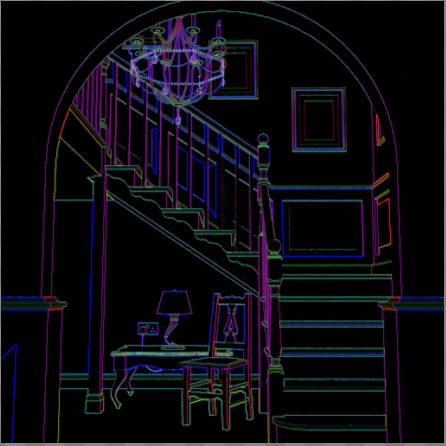
\includegraphics[width=45mm]{image/networkInput/normalV.png} \\
    color variance & albedo variance & normal variance
\end{tabular}
\end{figure}

Like in \cite{kuznetsov2018deep} and \cite{10.1145/3550454.3555515}, I divided the training
into three phases. In each phase, the batch size is 8, with the Adam optimiser \cite{kingma2017adam}
with $\epsilon = 10^{-4}$ for the gradient descent..
\begin{itemize}
    \item[1.] Train the denoiser $\D$ alone, with image perlin noise as sampling map: 
                40 000 iterations.
    \item[2.] Train the sampler $\Sm$ with a fixed denoiser: 20 000 iterations.
    \item[3.] Train jointly the denoiser $\D$ and the sampler $\Sm$: 20 000 iterations.
\end{itemize}
The full training took one day.

\paragraph*{Loss} I used the same loss function $\Los$ as in \cite{kuznetsov2018deep}.
\begin{equation}
    \label{eq:6}
    \Los(\hat c,c) = 0.5\Los_s(\hat c,c) + 0.5\Los_g(\hat c,c) 
\end{equation}
with a $Los_s$ is a $\ell_1$ loss to ensure the pixel have the right color:
\begin{equation}
    \label{eq:7}
    \Los_s(\hat c,c) = \frac{\lVert \log(1+\hat c) - \log(1+c) \rVert_1}{|c| + \epsilon}
\end{equation}
and with $Los_g$ is loss on the gradient to ensure the sharpness of the edge explain in \cite{5617283}.
\begin{equation}
    \label{eq:8}
    \Los_s(\hat c,c) = \frac{\lVert g(\log(1+\hat c)) - g(\log(1+c)) \rVert_1}{|c| + \epsilon}
\end{equation}

\subsection{Experimental result}

\paragraph*{Information} This section need still active work, 
I still have a full month to do a proper analysis, but
here is a less rigourus analysis of of result, as I have to send 
the report now, but a better analysis will be done in the futur.

In order to mesure if our sampler is working correctly, we can do two thing:
\begin{itemize}
    \item See if our sampler with our finetune denoiser is better that the base denoiser 
    that denoise a uniformly sample image.
    \item Compare our method that is specially adapted to stratified sampler, with DARS using stratified
    sampler. 
\end{itemize}
In order to have a fair comparaison, I trained DARS with the exact same dataset and with the same 
number of iteration.



\subsubsection{Comparaison to uniform sampling map {\color{red} TO DO}}


\subsubsection{Compariason to DARS {\color{red} TO DO}}


\section{Conclusion {\color{red} TODO}}


\printbibliography

\appendix

\section{Math tools}

\subsection{Combination of statistic} \label{combi}
As described in \cite{Chan1983AlgorithmsFC} we can combine statistics easly.
let $A$ be a set of sample and for $a\in A$, let $x_a$ be an observation. We note: 
\[E(A) = \frac{\sum_{a\in A} x_a}{|A|}, \qquad V(A) = \frac{\sum_{a\in A} (E(A) - x_a)^2}{|A|}\]
We then have the following formula to combine $A, B$ two set of sample:
\[E(A\cup B) = \frac{|A|\times I(A) + |B|\times I(B)}{|A|+|B|}\]
\[V(A\cup B) = \frac{ |A|\times V(A) + |B|\times V(B) + 
        \frac{|A||B|}{|A| + |B|}\left(E(A) - E(B)\right)}{|A| + |B|}\]

We can then inverse this equation to retreive the image using $B$ for the image
using $A$ and $A\cup B$. Here the formula in the spacial case where $|A| = |B|$:
\[ E(B) =  2 E(A\cup B) - E(A) \]
\[ V(B) =  2 V(A\cup B) - V(A) - 0.5[E(A\cup B) - E(A)]^2\]


\section{Image}

\subsection{Denoiser} \label{denoiserImage}

\begin{figure}[H]
    \centering
    \begin{tabular}{cccc}
    \includegraphics[width=80mm]{image/denoiser/noisy.png}
    & \includegraphics[width=80mm]{image/denoiser/kernelmap.png} \\
    noisy (2 spp) & kernelmap \\
    \includegraphics[width=80mm]{image/denoiser/denoisy.png}
    & \includegraphics[width=80mm]{image/denoiser/gt.png} \\
    denoisy & groundtruth \\
    \end{tabular}
\end{figure}

\end{document}